%%%%%%%%%%%%%%%%%%%%%%%%%%%%%%%%%%%%%%%%%%%%%%%%%%%%%%%%%%%%%%%%%%%%%%%%%%%%%%%
%\vspace{-2mm}
\chapter{RESULTADOS E DISCUSSÃO}

A presente seção apresenta e discute o resultado da aplicação da classe \texttt{LombScarbgle} do pacote \texttt{astropy} sobre os dados do fluxo solar F10.7. Mas antes, a Figura \ref{fig:original365} exibe o espectro de potência dos dados de média diárias do índice F10.7. Ele foi obtido via FFT conforme explicitado em \citeonline{Leo}. % aos três conjuntos de dados originais: dados de médias diárias, médias de 27 dias e médias anuais do índice solar F10.7 (Figura \ref{fig:original365}, \ref{fig:original12} e \ref{fig:original1}, respectivamente). O espectro de potência foi obtido conforme explicitado em \citeonline{Leo}. 

\vspace{-8mm}
\begin{figure}[ht!]
	\caption{Espectro de potência dos dados originais (média diária).}
	\vspace{1mm}	% acrescentar o espaçamento vertical apropriado entre o título e a borda superior da figura
	\begin{center}
		\resizebox{.7\textwidth}{!}{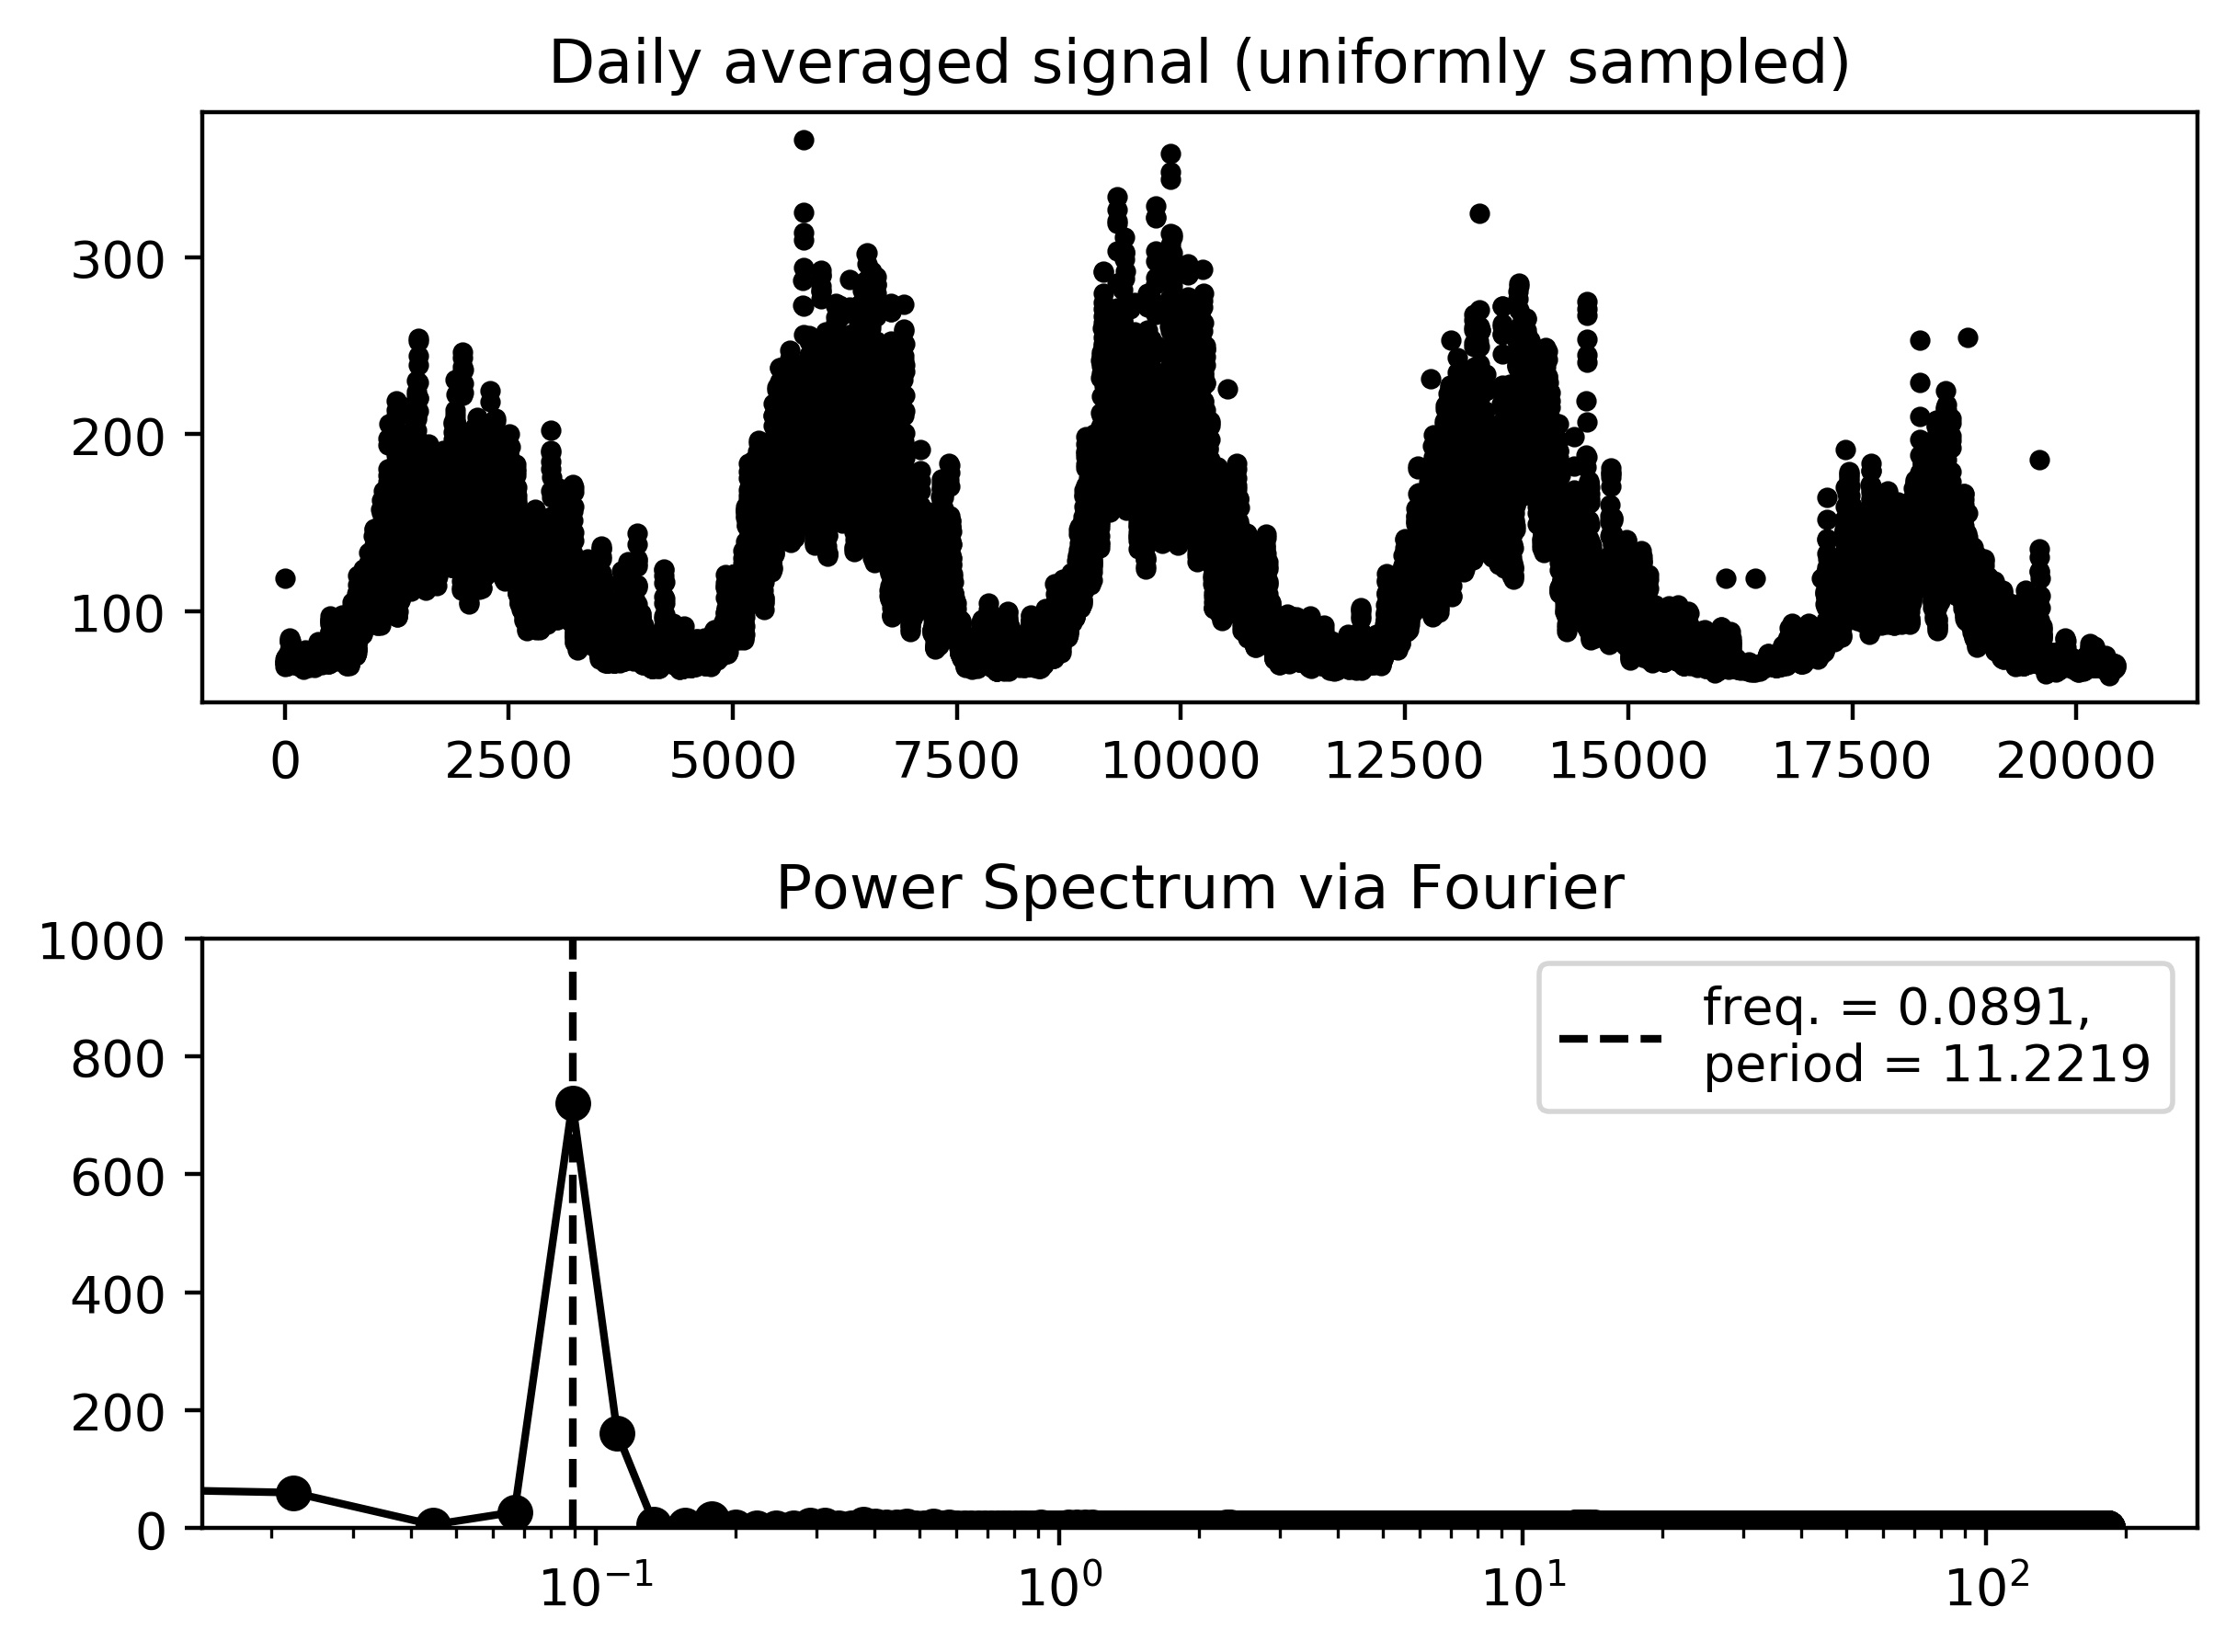
\includegraphics{Figuras/original_365.jpg}}
	\end{center}
	\vspace{-1mm}	% acrescentar o espaçamento vertical apropriado entre a borda inferior da figura e a legenda ou a fonte quando não há legenda (o valor pode ser negativo para subir)
	\legenda{Espectro de potência via FFT das médias diárias do índice  solar F10.7. Com amostragem uniforme, longa janela de observação e sampling rate satisfatório, a técnica do espectro de Fourier via algoritmos de FFT é um método robusto e amplamente empregado.}	% legenda - para deixar sem legenda usar comando \legenda{} (nunca deve-se comentar o comando \legenda)
	\label{fig:original365}
	%\FONTE{\url{https://omniweb.gsfc.nasa.gov/form/dx1.html}.}	% fonte consultada (elemento obrigatório, mesmo que seja produção do próprio autor)
\end{figure}

%\begin{figure}[ht!]
%	\caption{Espectro de potência dos dados originais (média de 27 dias).}
%	\vspace{1mm}	% acrescentar o espaçamento vertical apropriado entre o título e a borda superior da figura
%	\begin{center}
%		\resizebox{.8\textwidth}{!}{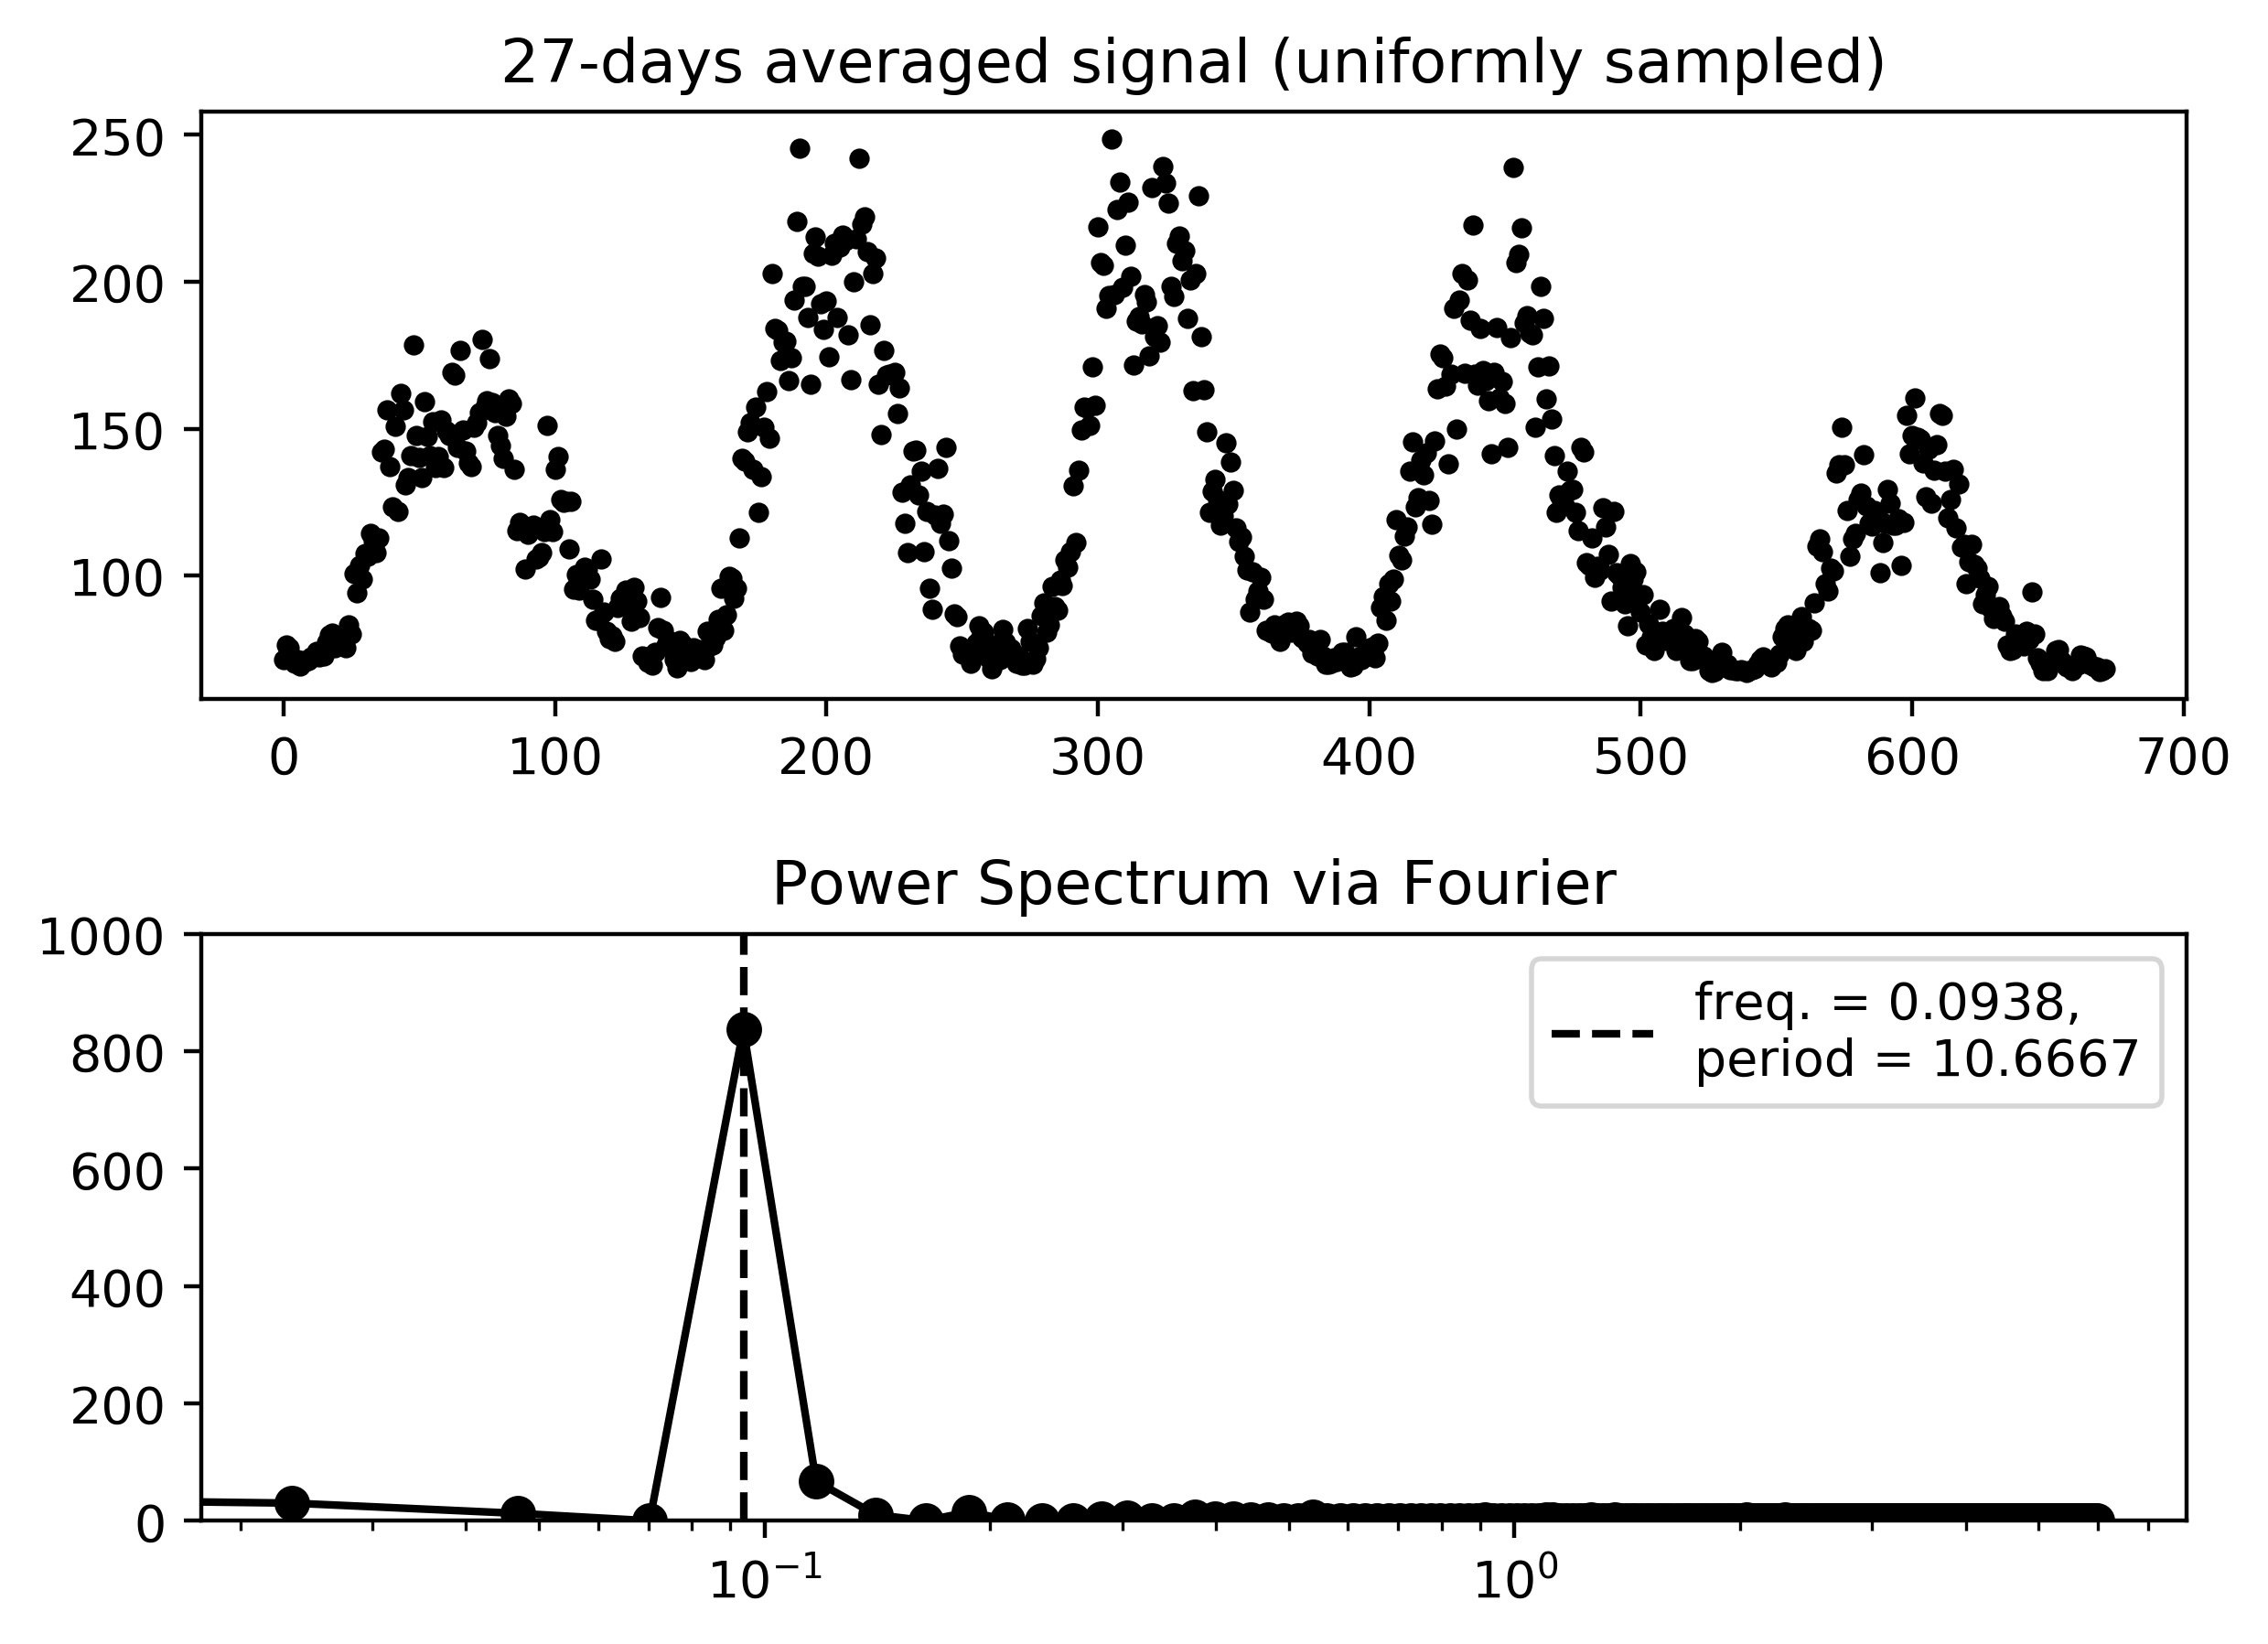
\includegraphics{Figuras/original_12.jpg}}
%	\end{center}
%	\vspace{-1mm}	% acrescentar o espaçamento vertical apropriado entre a borda inferior da figura e a legenda ou a fonte quando não há legenda (o valor pode ser negativo para subir)
%	\legenda{Aplicação do espectro de Fourier sobre as médias de 27 dias do índice  solar F10.7 sob amostragem uniforme. Novamente a análise de Fourier pode ser empregada sem problemas.}	% legenda - para deixar sem legenda usar comando \legenda{} (nunca deve-se comentar o comando \legenda)
%	\label{fig:original12}
	%\FONTE{\url{https://omniweb.gsfc.nasa.gov/form/dx1.html}.}	% fonte consultada (elemento obrigatório, mesmo que seja produção do próprio autor)
%\end{figure}

%\begin{figure}[ht!]
%	\vspace{-20mm}	
%	\caption{Espectro de potência dos dados originais (média anual).}
%	\vspace{1mm}	% acrescentar o espaçamento vertical apropriado entre o título e a borda superior da figura
%	\begin{center}
%		\resizebox{.8\textwidth}{!}{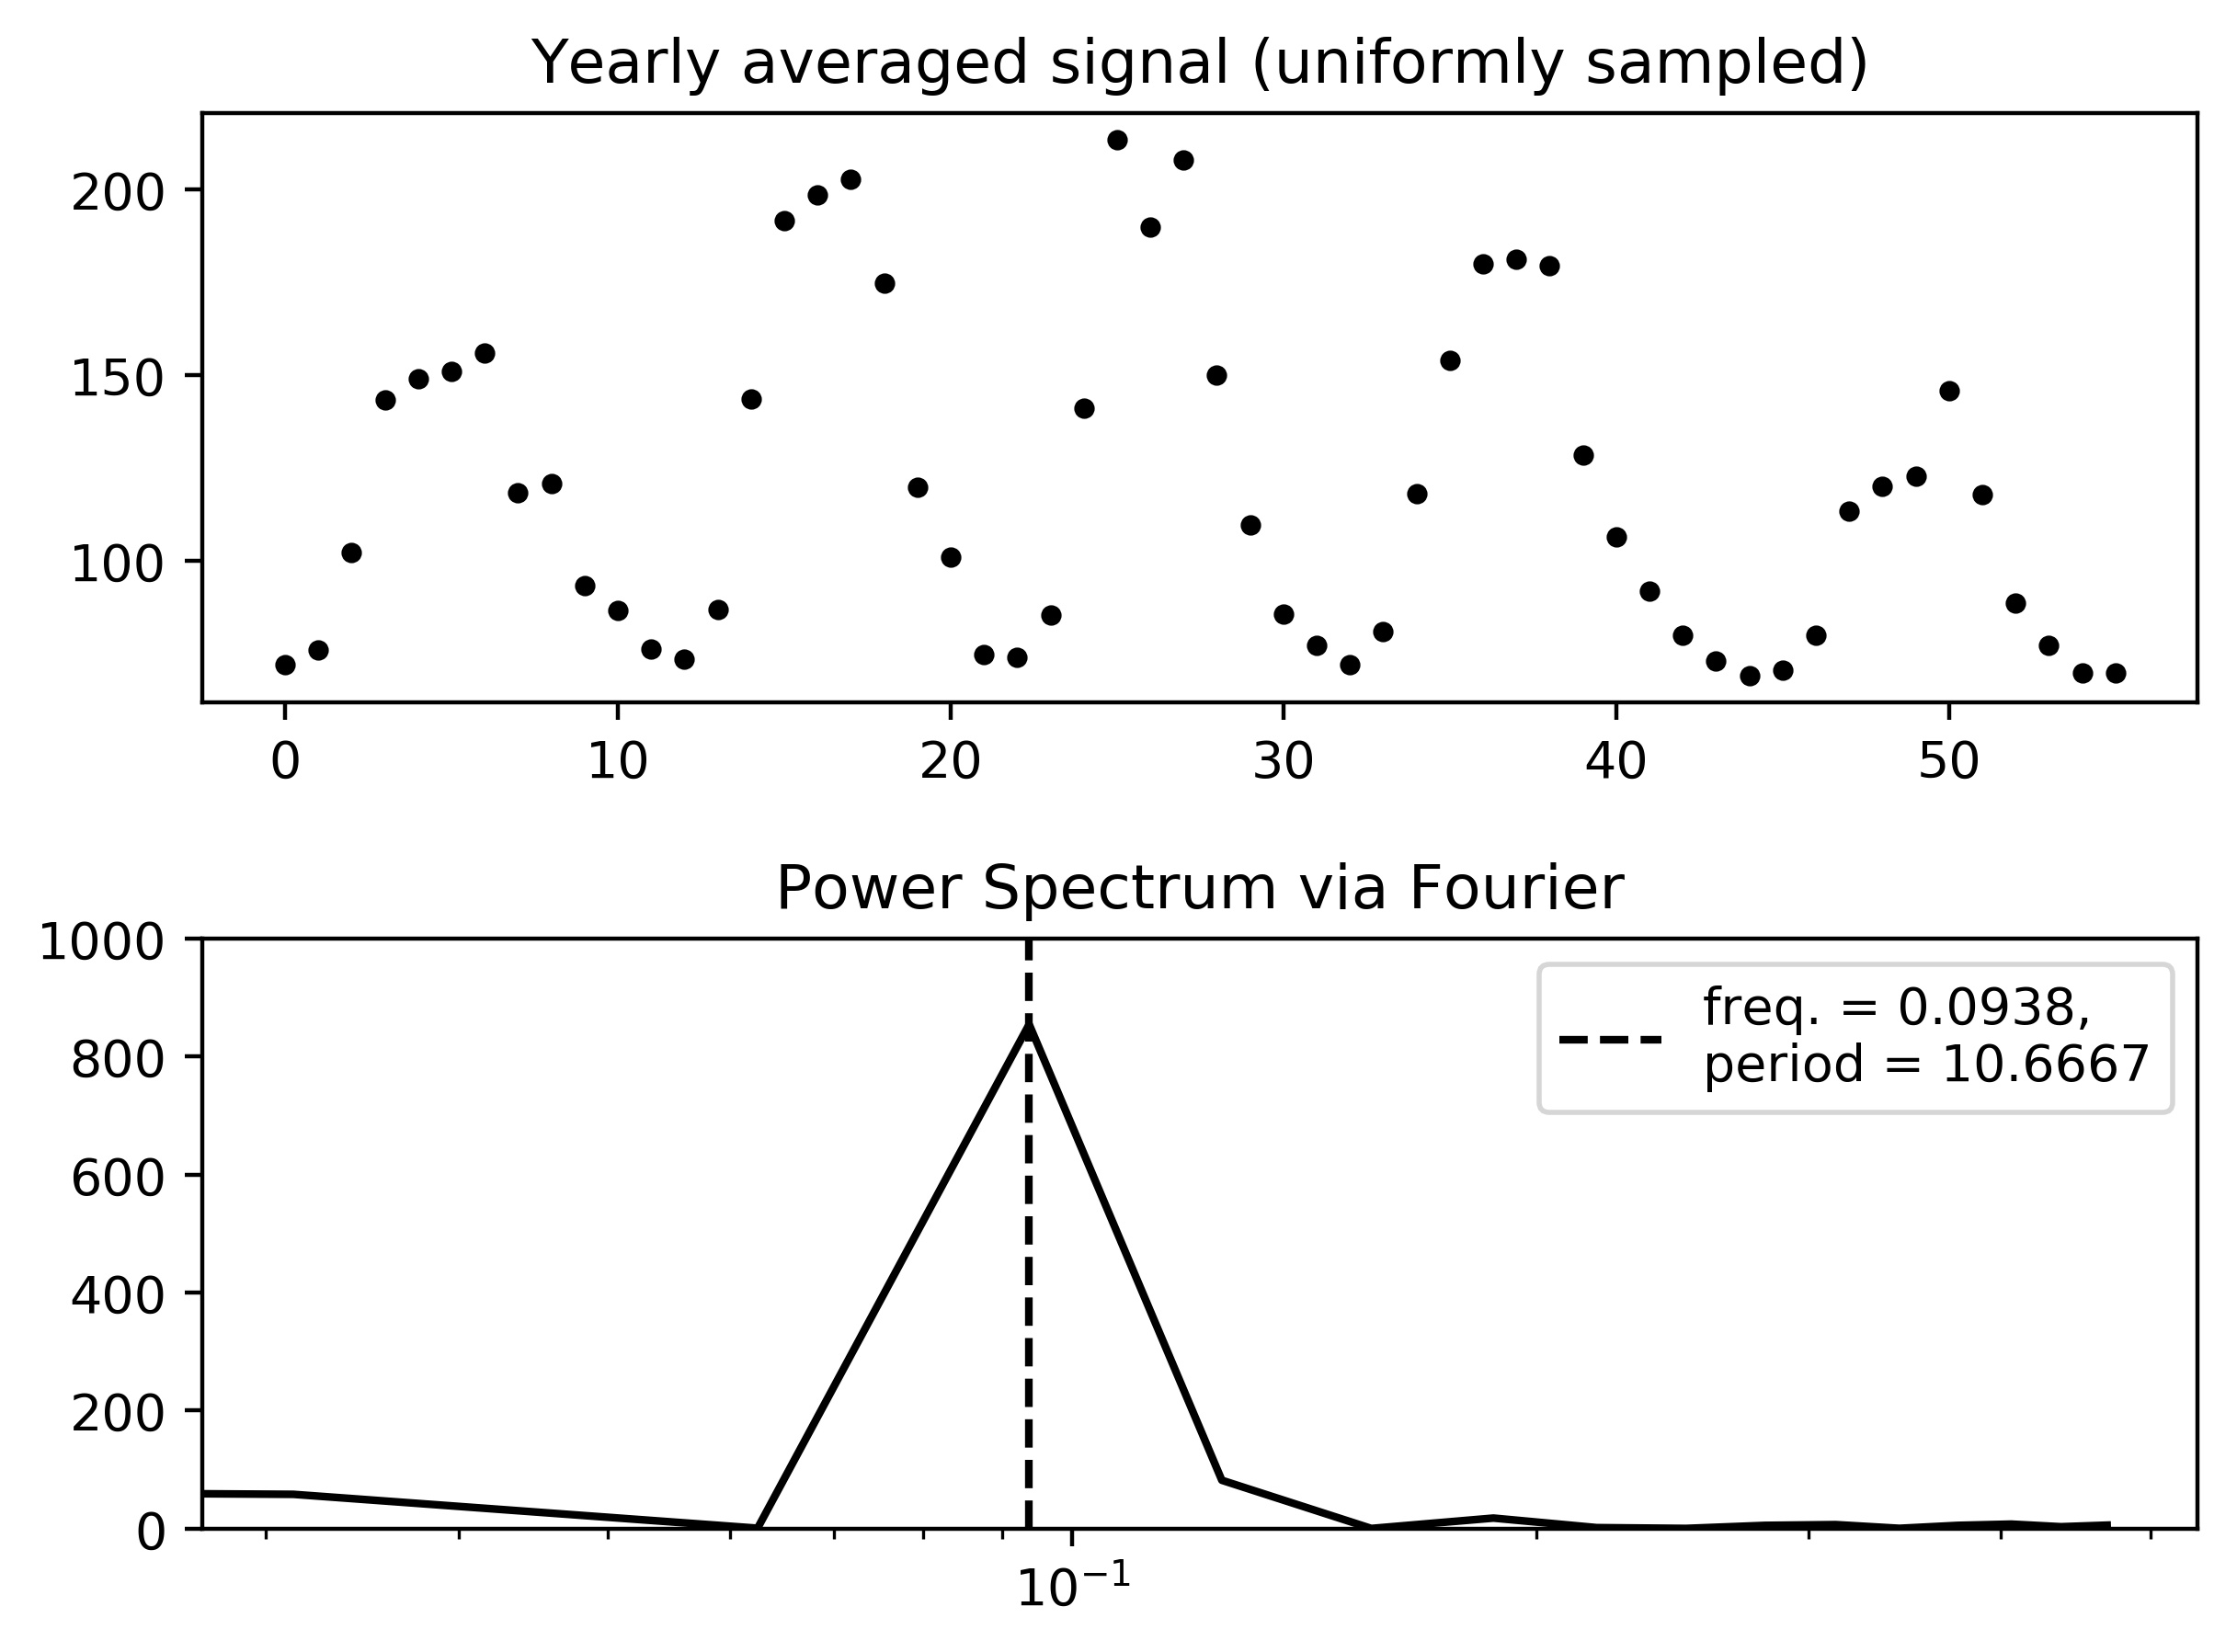
\includegraphics{Figuras/original_1.jpg}}
%	\end{center}
%	\vspace{-1mm}	% acrescentar o espaçamento vertical apropriado entre a borda inferior da figura e a legenda ou a fonte quando não há legenda (o valor pode ser negativo para subir)
%	\legenda{Aplicação do espectro de Fourier sobre as médias anuais do índice  solar F10.7. A amostragem novamente é uniforme, porém com taxa muito inferior à dos demais conjuntos de dados. Ainda assim o espectro de potência via Fourier se mostra uma ferramenta poderosa.}	% legenda - para deixar sem legenda usar comando \legenda{} (nunca deve-se comentar o comando \legenda)
%	\label{fig:original365}
	%\FONTE{\url{https://omniweb.gsfc.nasa.gov/form/dx1.html}.}	% fonte consultada (elemento obrigatório, mesmo que seja produção do próprio autor)
%\end{figure}

\clearpage{}
Nas seções a seguir, os dados de médias diárias do fluxo F10.7 são investigados sob diferentes cenários de amostragem aleatória. O primeiro cenário se baseia em gaps (intervalos) de interrupção na aquisição dos dados. São testados cinco números de gaps diferentes, posicionados aleatoriamente e com o mesmo tamanho. O segundo cenário simula a ausência aleatória dos dados, considerando cinco porcentagens diferentes do tamanho inicial da amostra para exclusão. Em todos os casos o resultado e a performance da classe \texttt{LombScargle} do pacote \texttt{astropy} são discutidos. A heurística da ferramenta foi configurada com \texttt{nyquist\_factor} $=$ 2 durante os testes.

\section{Cenário 1 - diferentes intervalos de observação}

Aqui são apresentados os resultados do periodograma de Lomb-Scargle para o cenário de interrupção de observação com intervalos aleatoriamente posicionados nos dados. Em todos os testes o intervalo tem tamanho fixo e igual a 10\% to tamanho da série total. A seguir são exibidos as figuras referentes às médias diárias do índice F10.7. %Os demais resultados estão disponíveis em LINK DO REPOSITÓRIO.

%\subsection{Médias diárias}

\begin{figure}[ht!]
\vspace{-7mm}	
	\caption{Análise das médias diárias com 4 intervalos.}
	\vspace{1mm}	
	\begin{center}
		\resizebox{.8\textwidth}{!}{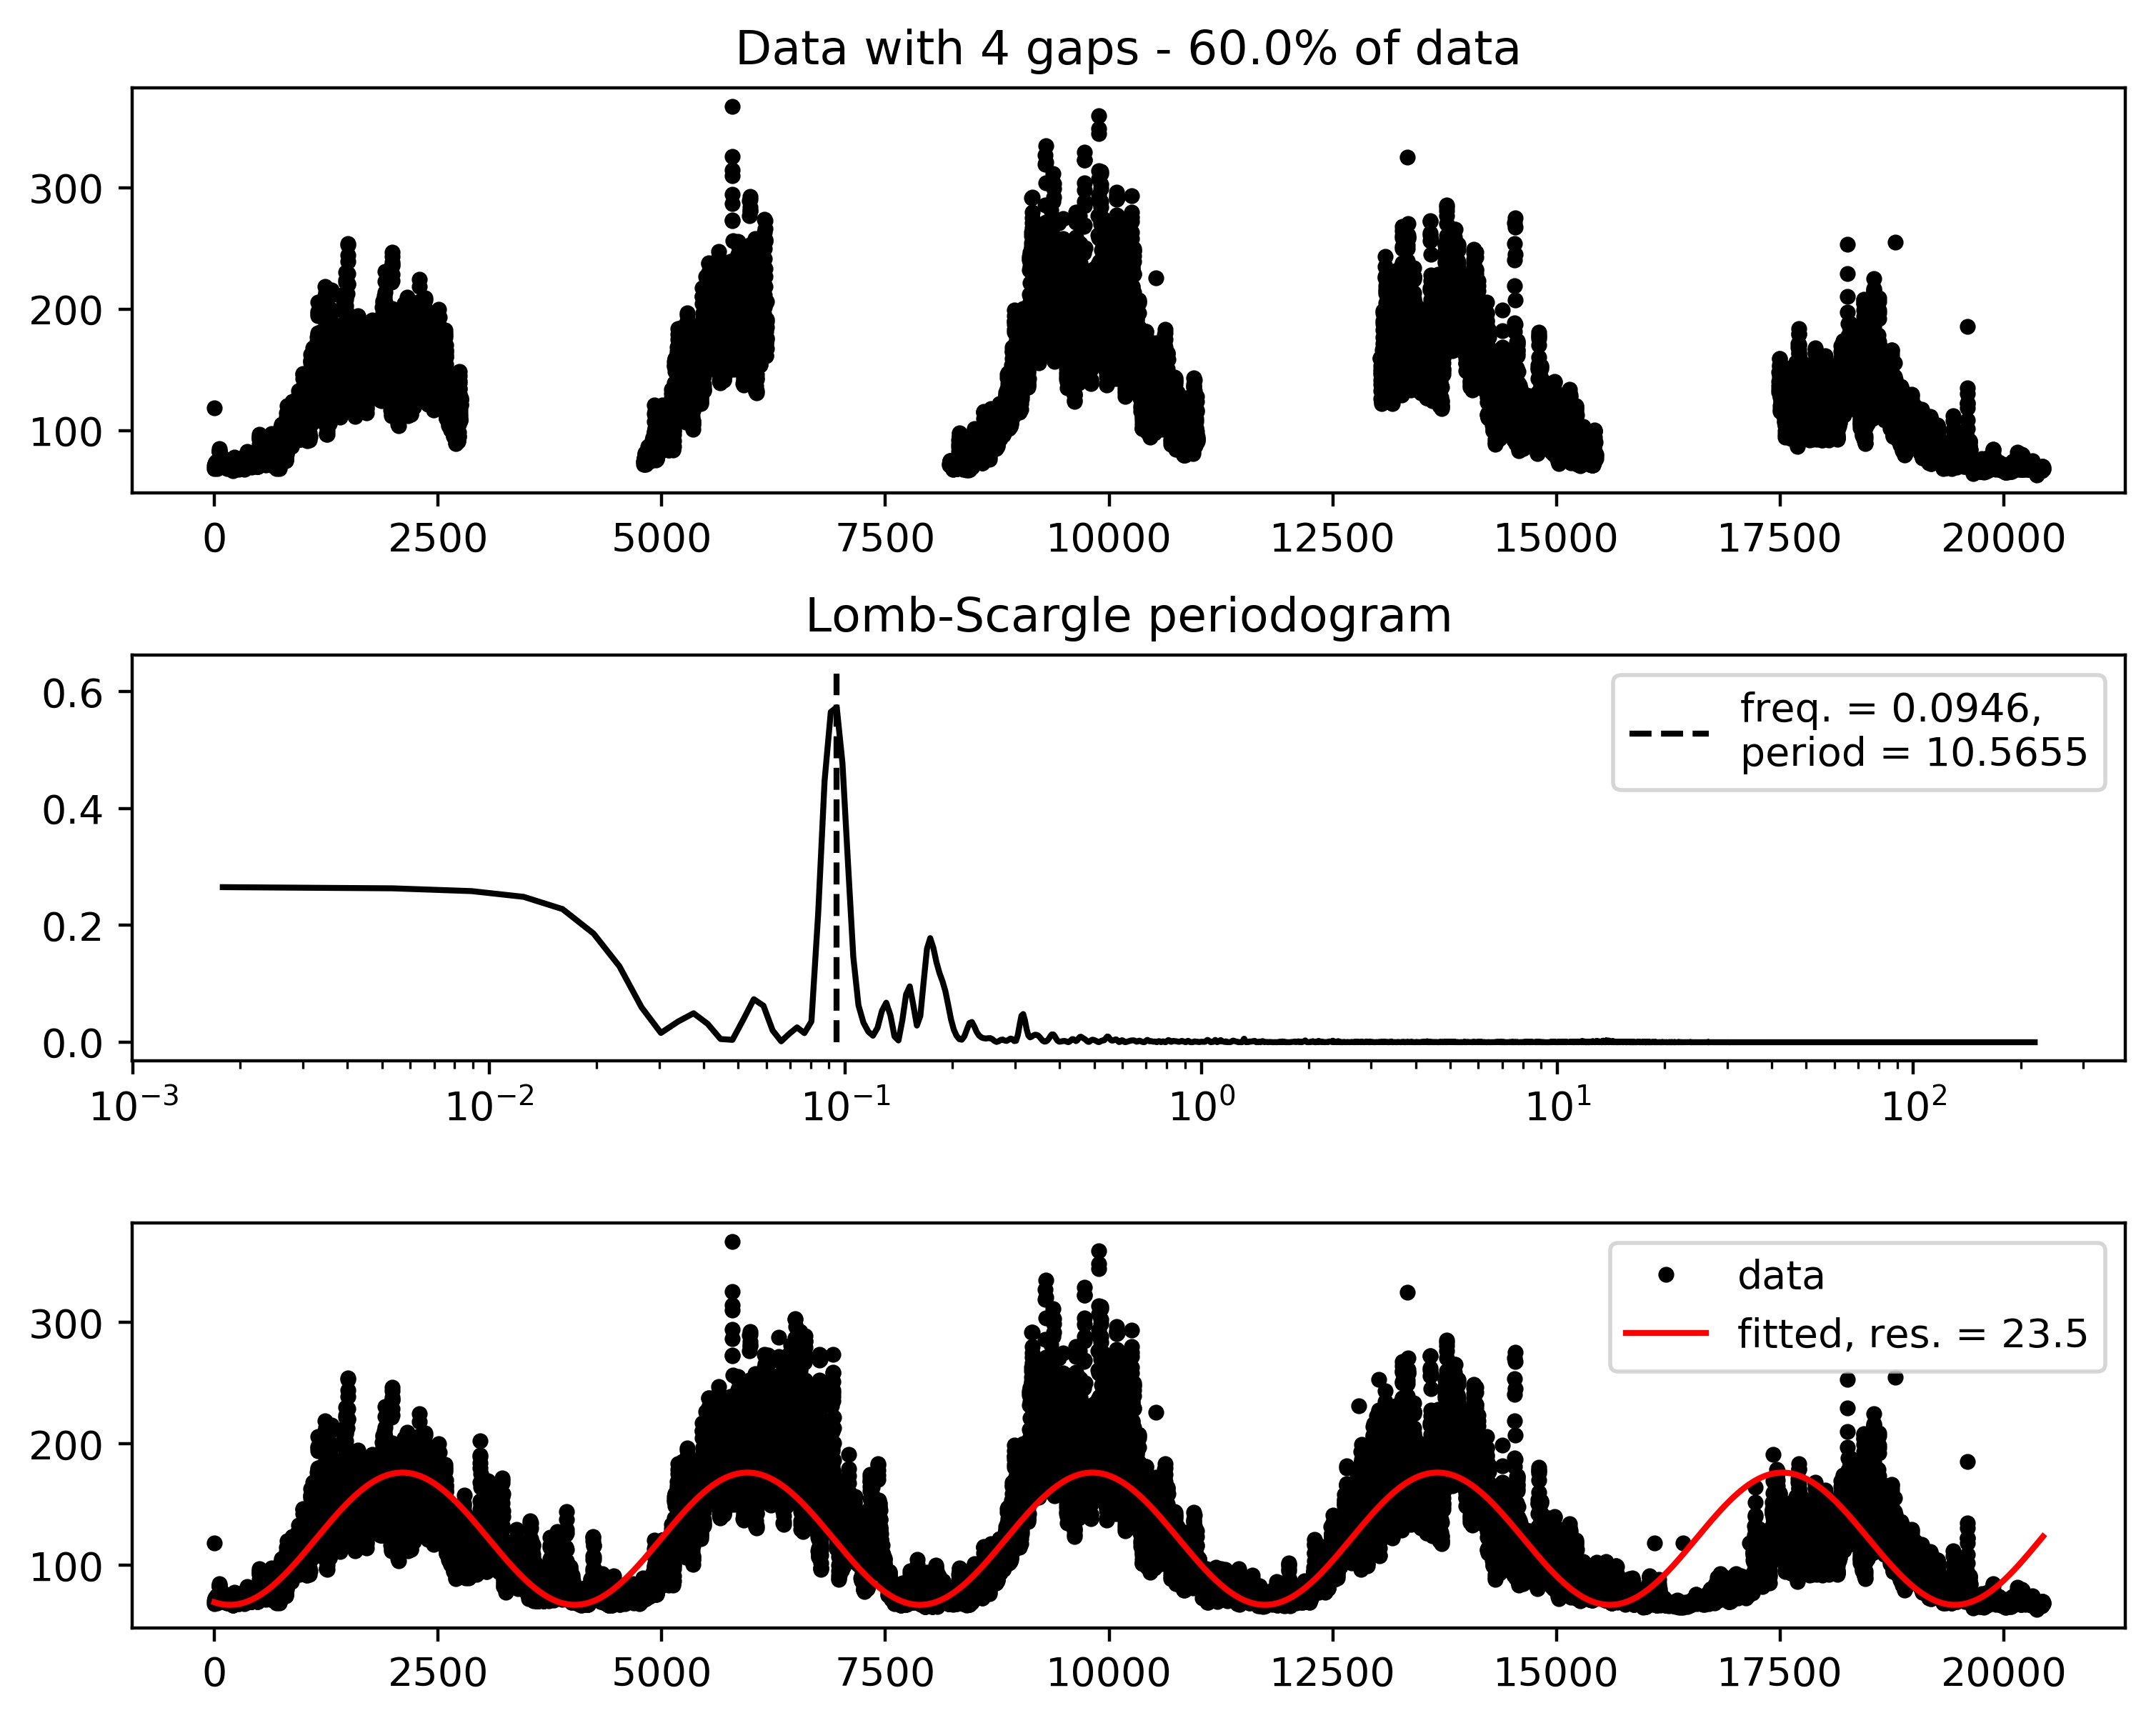
\includegraphics{../scripts/dataset1/periodograms_ny2.0_model2_Ng4.jpg}}
	\end{center}
	\vspace{-1mm}	
	\legenda{Topo: série de médias diárias do fluxo 10.7 com a presença de 4 gaps na obtenção de dados, restando assim 60\% dos dados originais. Meio: periodograma de Lomb-Scargle com indicação da frequência predominante determinada pela localização do pico. Abaixo: em preto a série original, em vermelho a senóide determinada a partir do método \texttt{model()}. O resíduo médio é indicado, quantificando o quanto a função ajustada pelo pacote \texttt{LombScargle} se aproxima da série original.}
	\label{fig:4gaps}
\end{figure}

\begin{figure}[ht!]
\vspace{-10mm}	
	\caption{Análise das médias diárias com 5 intervalos.}
	\vspace{1mm}	
	\begin{center}
		\resizebox{.8\textwidth}{!}{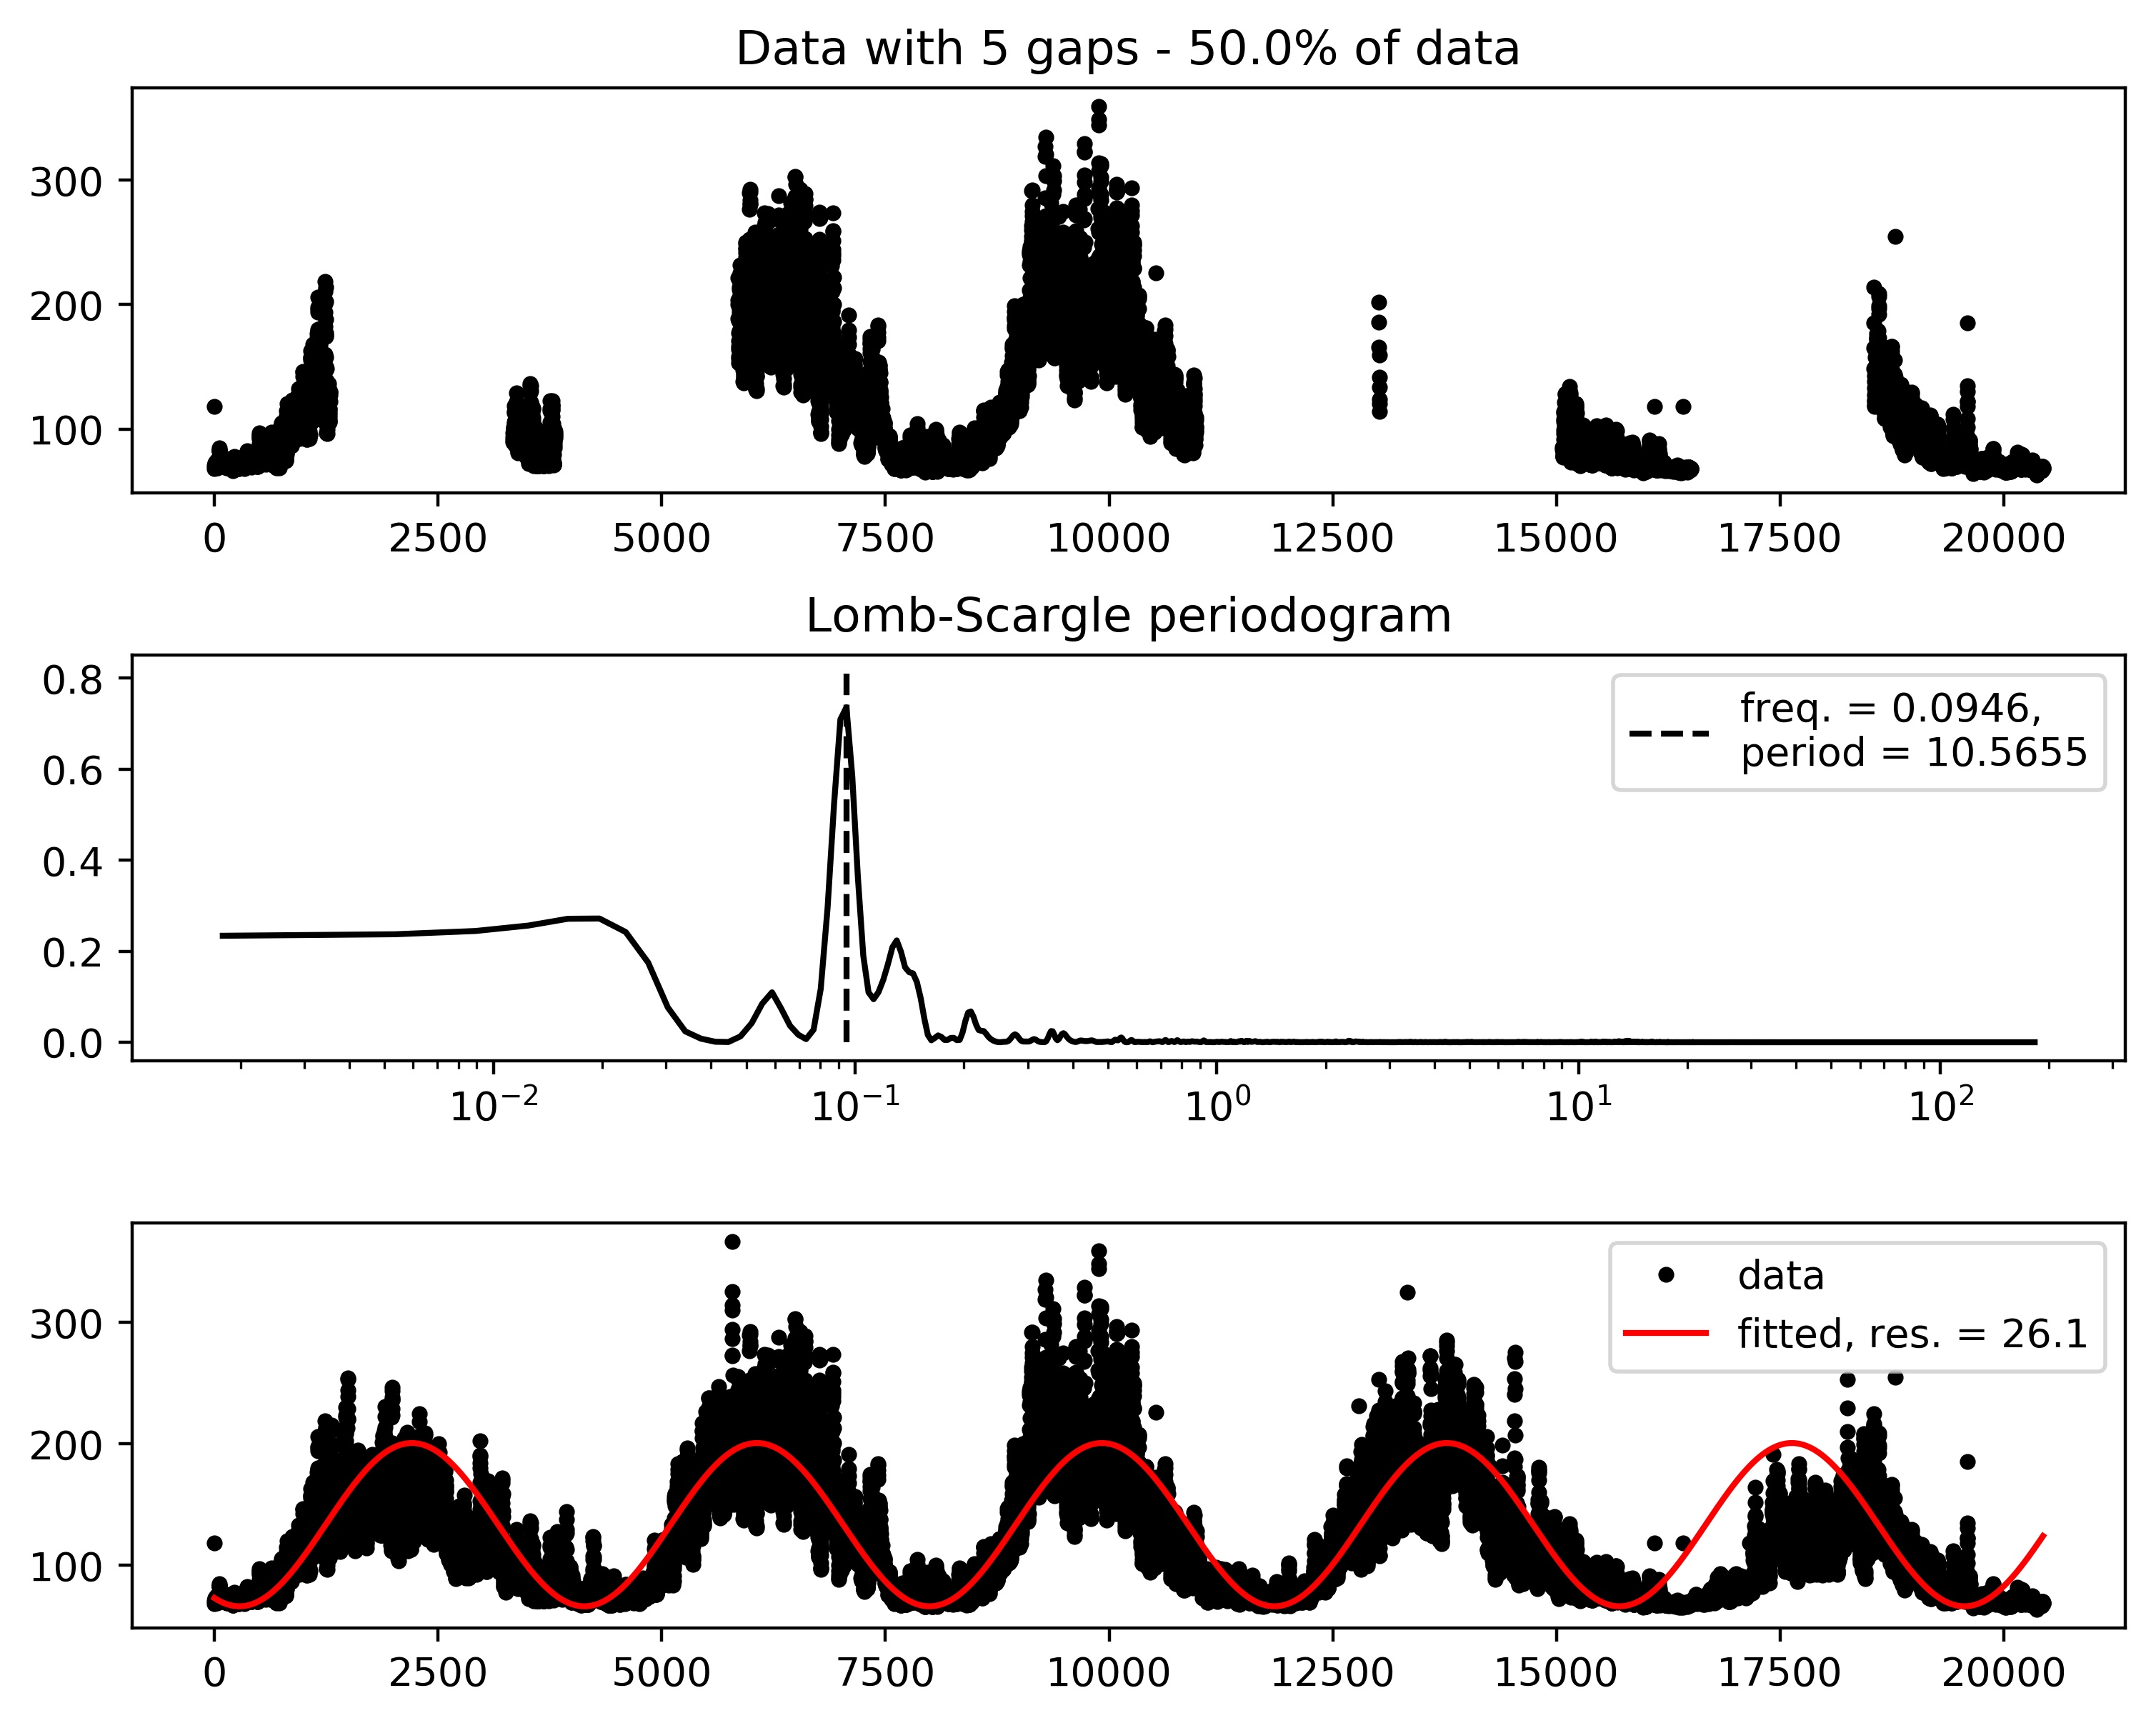
\includegraphics{../scripts/dataset1/periodograms_ny2.0_model2_Ng5.jpg}}
	\end{center}
	\vspace{-1mm}	
	\legenda{Resultado para 5 intervalos. Novamente a ferramenta utilizada corretamente identificou a periodicidade do sinal, e a função ajustada também corresponde bem à série original.}
	\label{fig:5gaps}
\end{figure}

\begin{figure}[ht!]
\vspace{-12mm}	
	\caption{Análise das médias diárias com 6 intervalos.}
	\vspace{1mm}	
	\begin{center}
		\resizebox{.8\textwidth}{!}{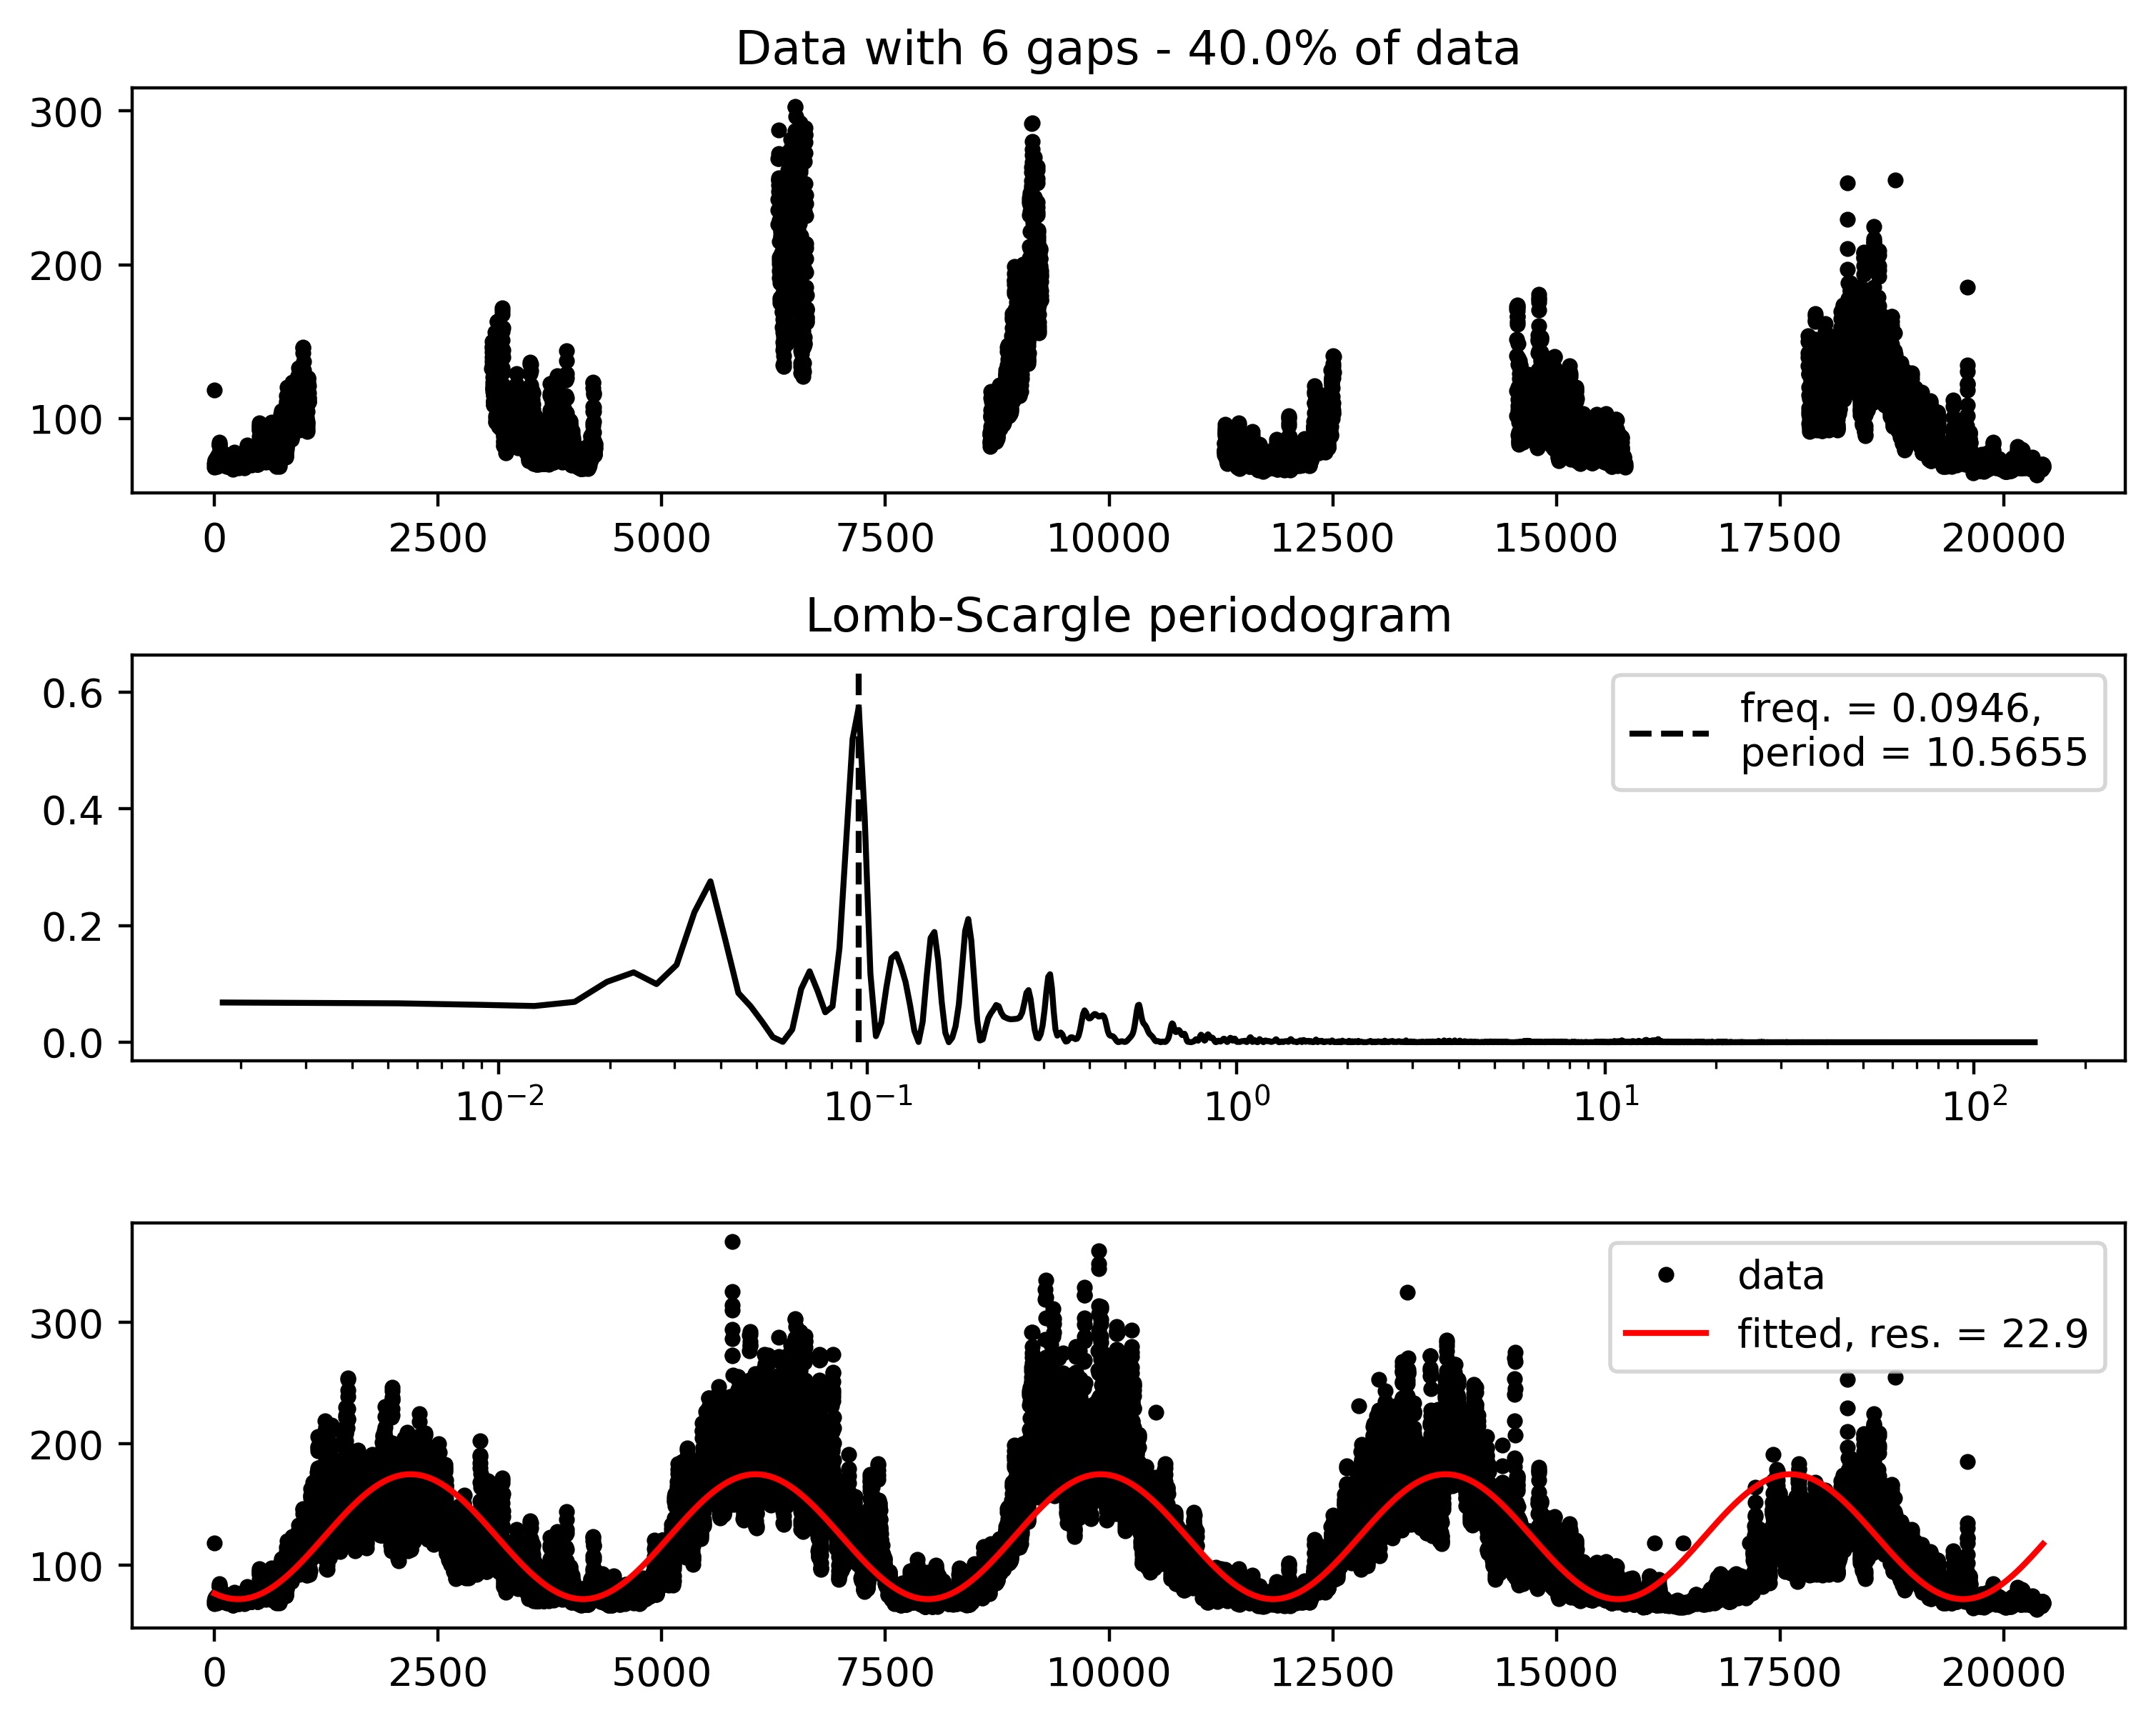
\includegraphics{../scripts/dataset1/periodograms_ny2.0_model2_Ng6.jpg}}
	\end{center}
	\vspace{-1mm}	
	\legenda{Resultado para 6 intervalos. Aqui mais frequências espúrias começam a surgir no periodograma, mas a principal assinatura ainda é bem identificada.}
	\label{fig:6gaps}
\end{figure}

\begin{figure}[ht!]
\vspace{-10mm}	
	\caption{Análise das médias diárias com 7 intervalos.}
	\vspace{1mm}	
	\begin{center}
		\resizebox{.8\textwidth}{!}{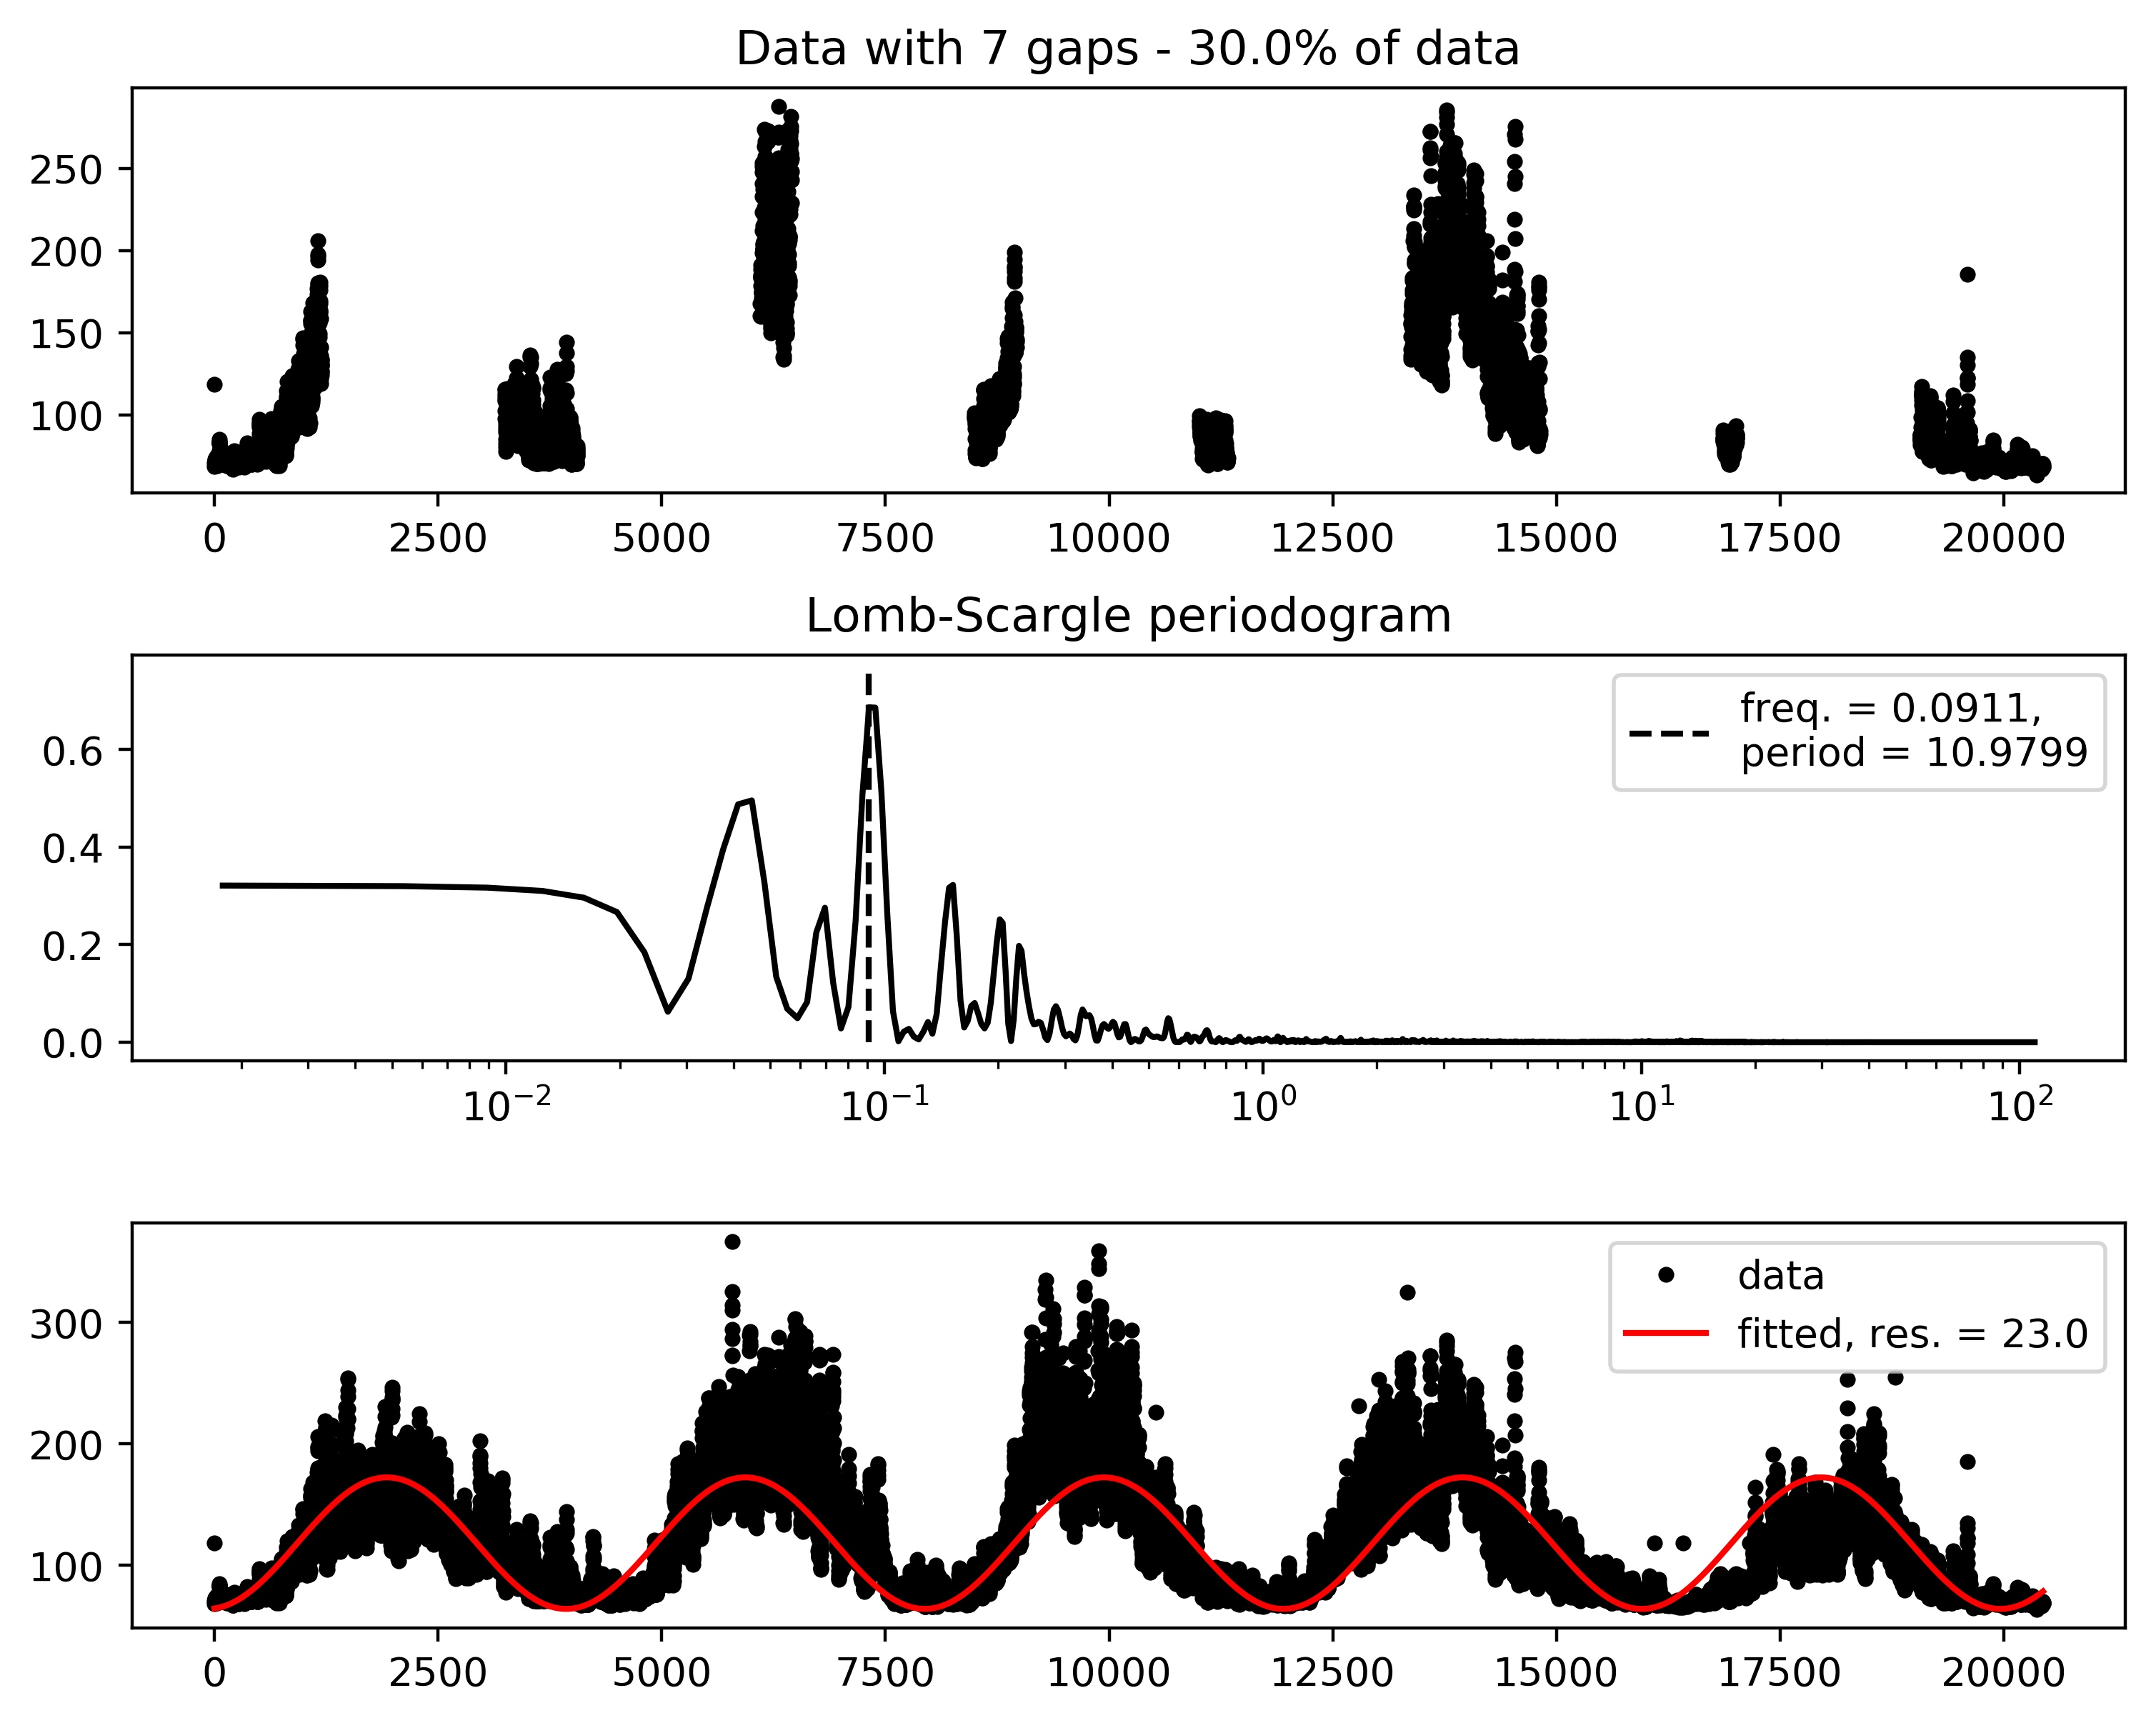
\includegraphics{../scripts/dataset1/periodograms_ny2.0_model2_Ng7.jpg}}
	\end{center}
	\vspace{-1mm}	
	\legenda{Resultado para 7 intervalos. Mesmo com somente 30\% dos dados, o resultado do periodograma de Lomb-Scargle se mostra consistente.}
	\label{fig:7gaps}
\end{figure}

\begin{figure}[ht!]
\vspace{-8mm}	
	\caption{Análise das médias diárias com 8 intervalos.}
	\vspace{1mm}	
	\begin{center}
		\resizebox{.8\textwidth}{!}{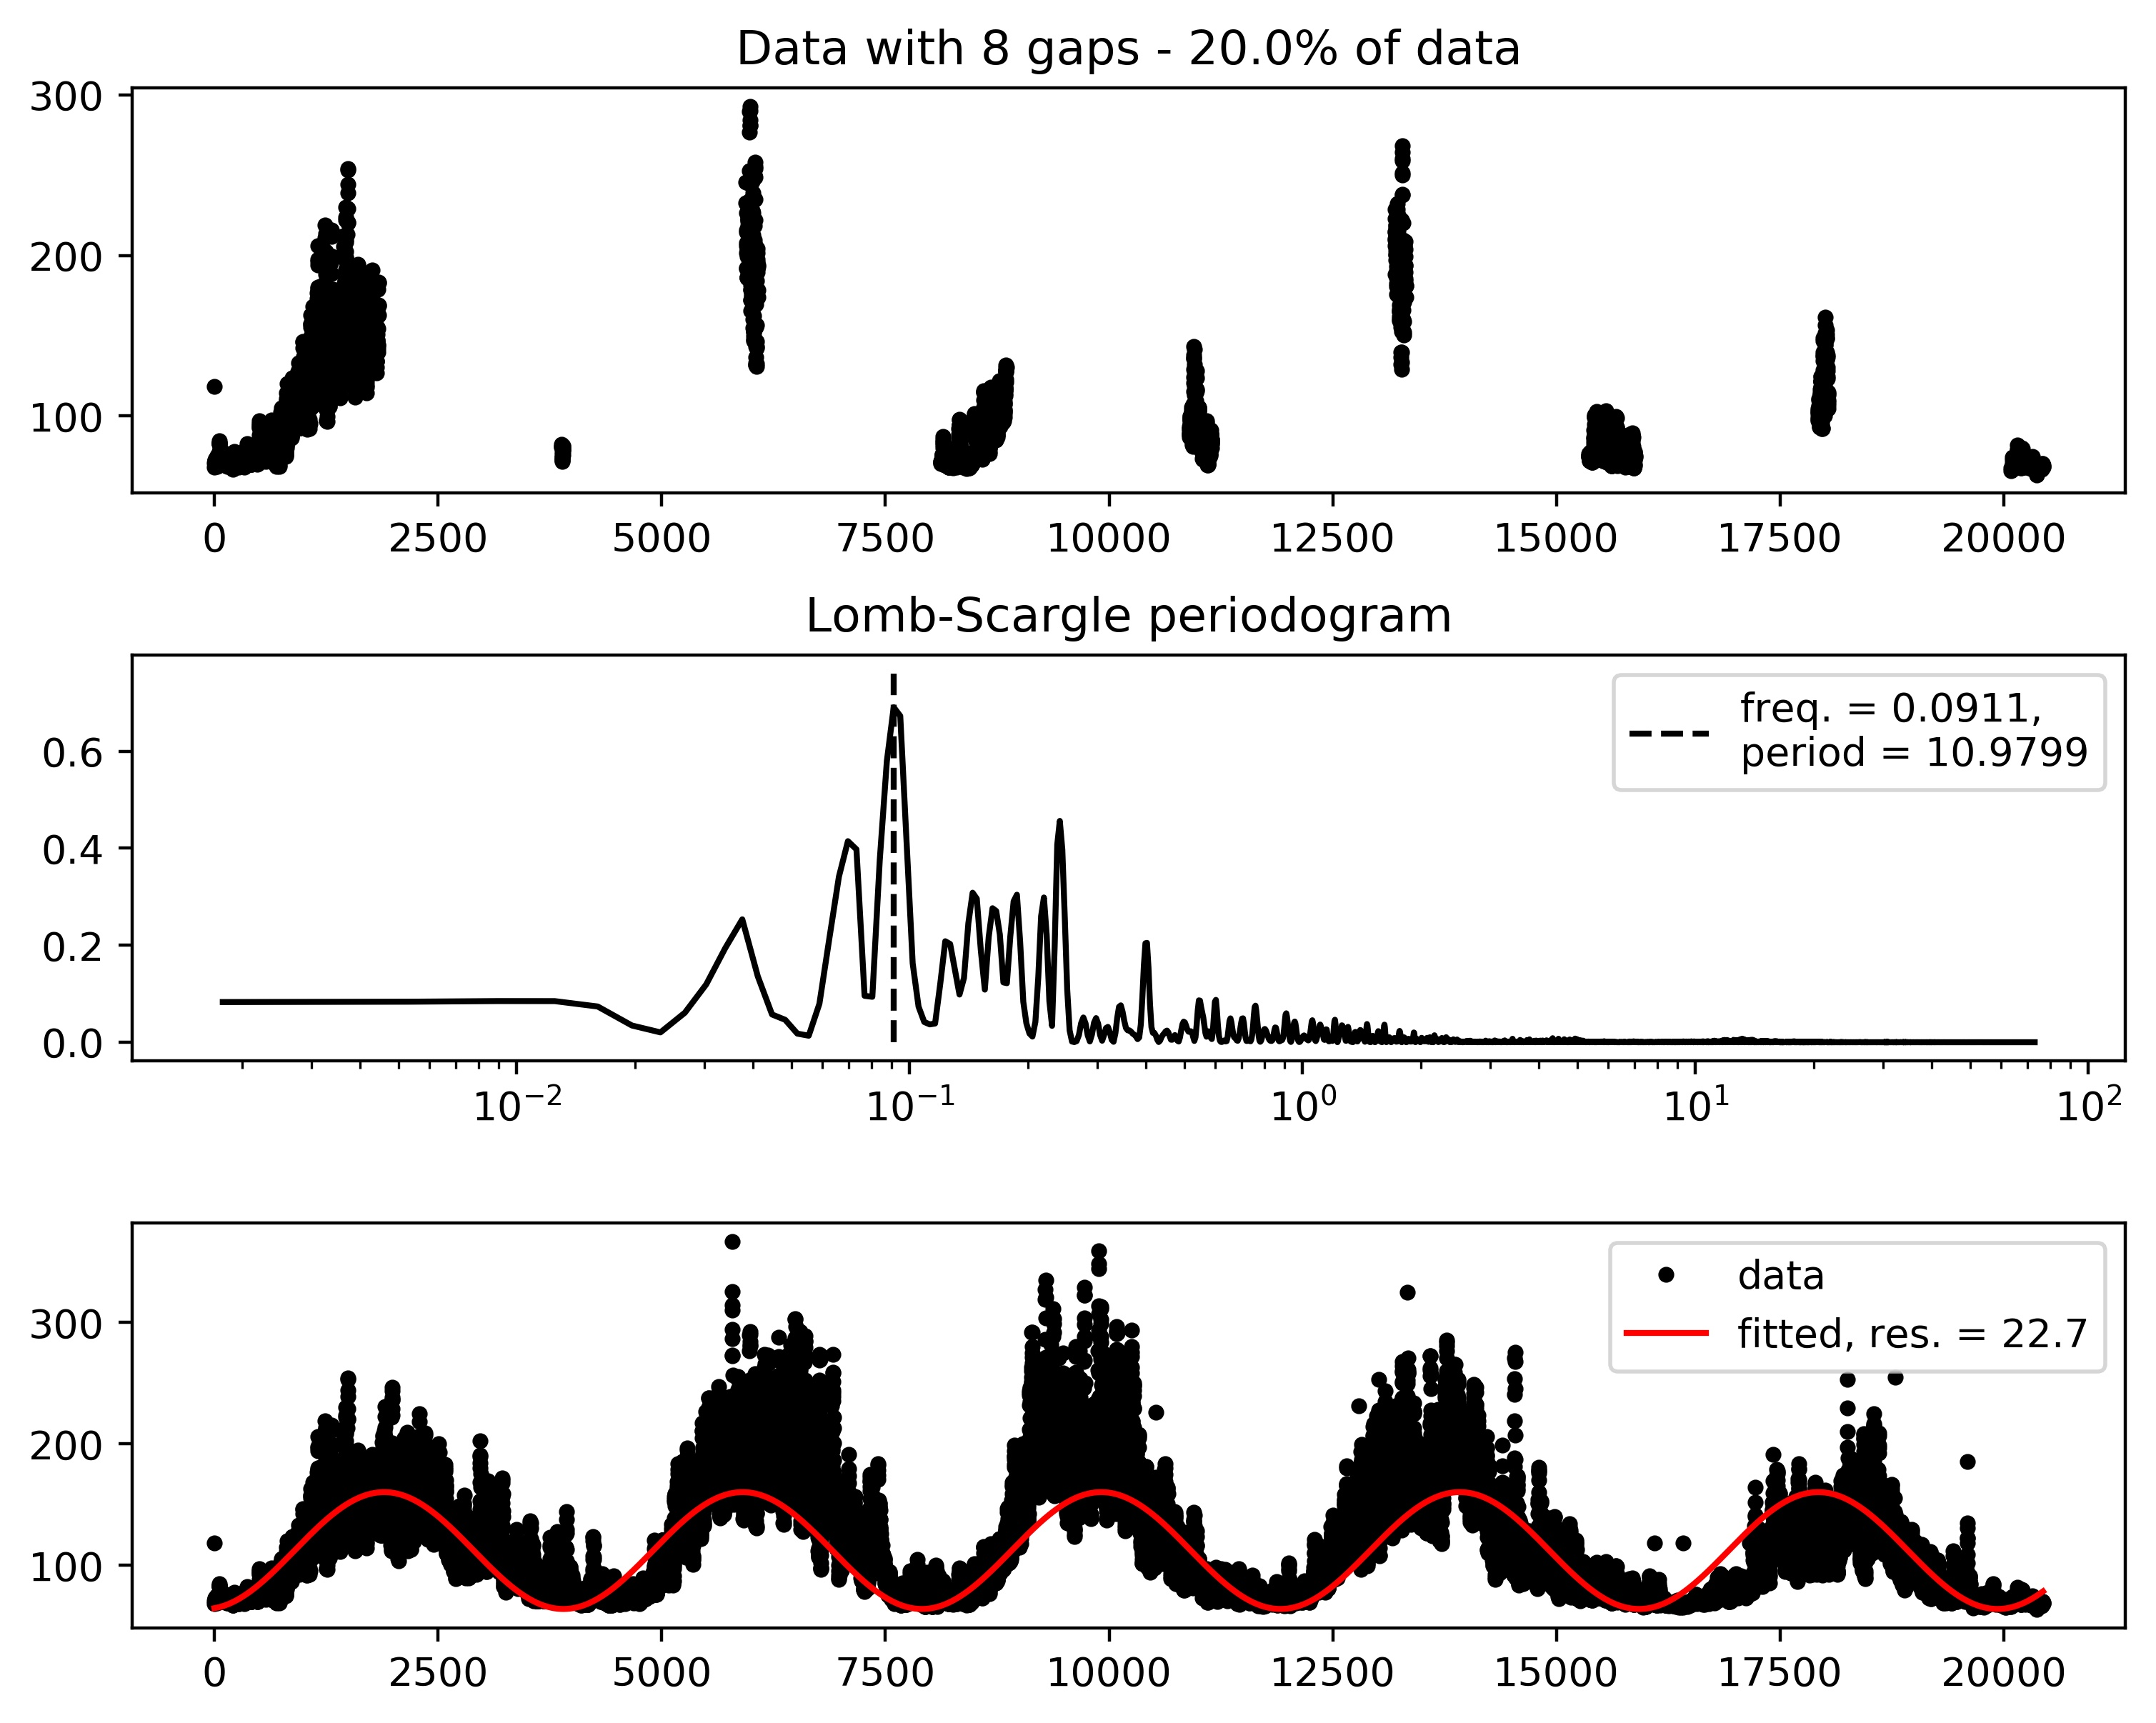
\includegraphics{../scripts/dataset1/periodograms_ny2.0_model2_Ng8.jpg}}
	\end{center}
	\vspace{-1mm}	
	\legenda{Resultado para 8 intervalos. A quantidade de picos espúrios próximo ao principal é maior que nos testes anteriores.}
	\label{fig:8gaps}
\end{figure}

\clearpage{}
\vspace*{-60px}	
Os resultados das Figuras \ref{fig:4gaps} a \ref{fig:8gaps} indicam que o periodograma de Lomb-Scargle é satisfatório em diversas situações de ausência de dados. A princípio, a Figura \ref{fig:4gaps} indica que a presença de poucos intervalos, tomando $\sim$40\% dos dados, não causa tantas anomalias ao periodograma. Os picos próximos ao principal (em 0.0946) são frequência que também se ajustaram bem aos dados. O resultado da melhor frequência foi aproximadamente o mesmo em todos os testes. Ao mesmo tempo, quanto maior o número de intervalos, maior foi a presença de picos espúrios. Neste sentido, as Figuras \ref{fig:7gaps} e \ref{fig:8gaps} ilustram uma característica (aleatória) do experimento: não só a quantidade de gaps, mas também a distribuição destes afetou a performance da ferramenta \texttt{LombScargle}, ainda que em menor grau. Ou seja, dependendo da posição dos intervalos durante um teste, os resultados com 6, 7 e 8 intervalos podiam ser igualmente bons, ruins, ou diferir substancialmente, mas sempre apresentando mais picos espúrios que os resultados com 4 ou 5 intervalos.

	
\section{Cenário 2 - exclusão aleatória de dados}
		
O cenário testado a seguir se baseia na exclusão aleatória das amostras até que se chegue a um limite estabelecido de porcentagem do total inicial. Esse limite foi variado cinco vezes, de modo que restasse entre 1\% e 0.04\% dos dados de média diária do fluxo 10.7. %Demais resultados estão presentes em LINK DO REPOSITORIO.

\begin{figure}[ht!]
\vspace{-10mm}	
	\caption{Análise com exclusão aleatória até 1\% dos dados.}
	\vspace{0mm}	
	\begin{center}
		\resizebox{.8\textwidth}{!}{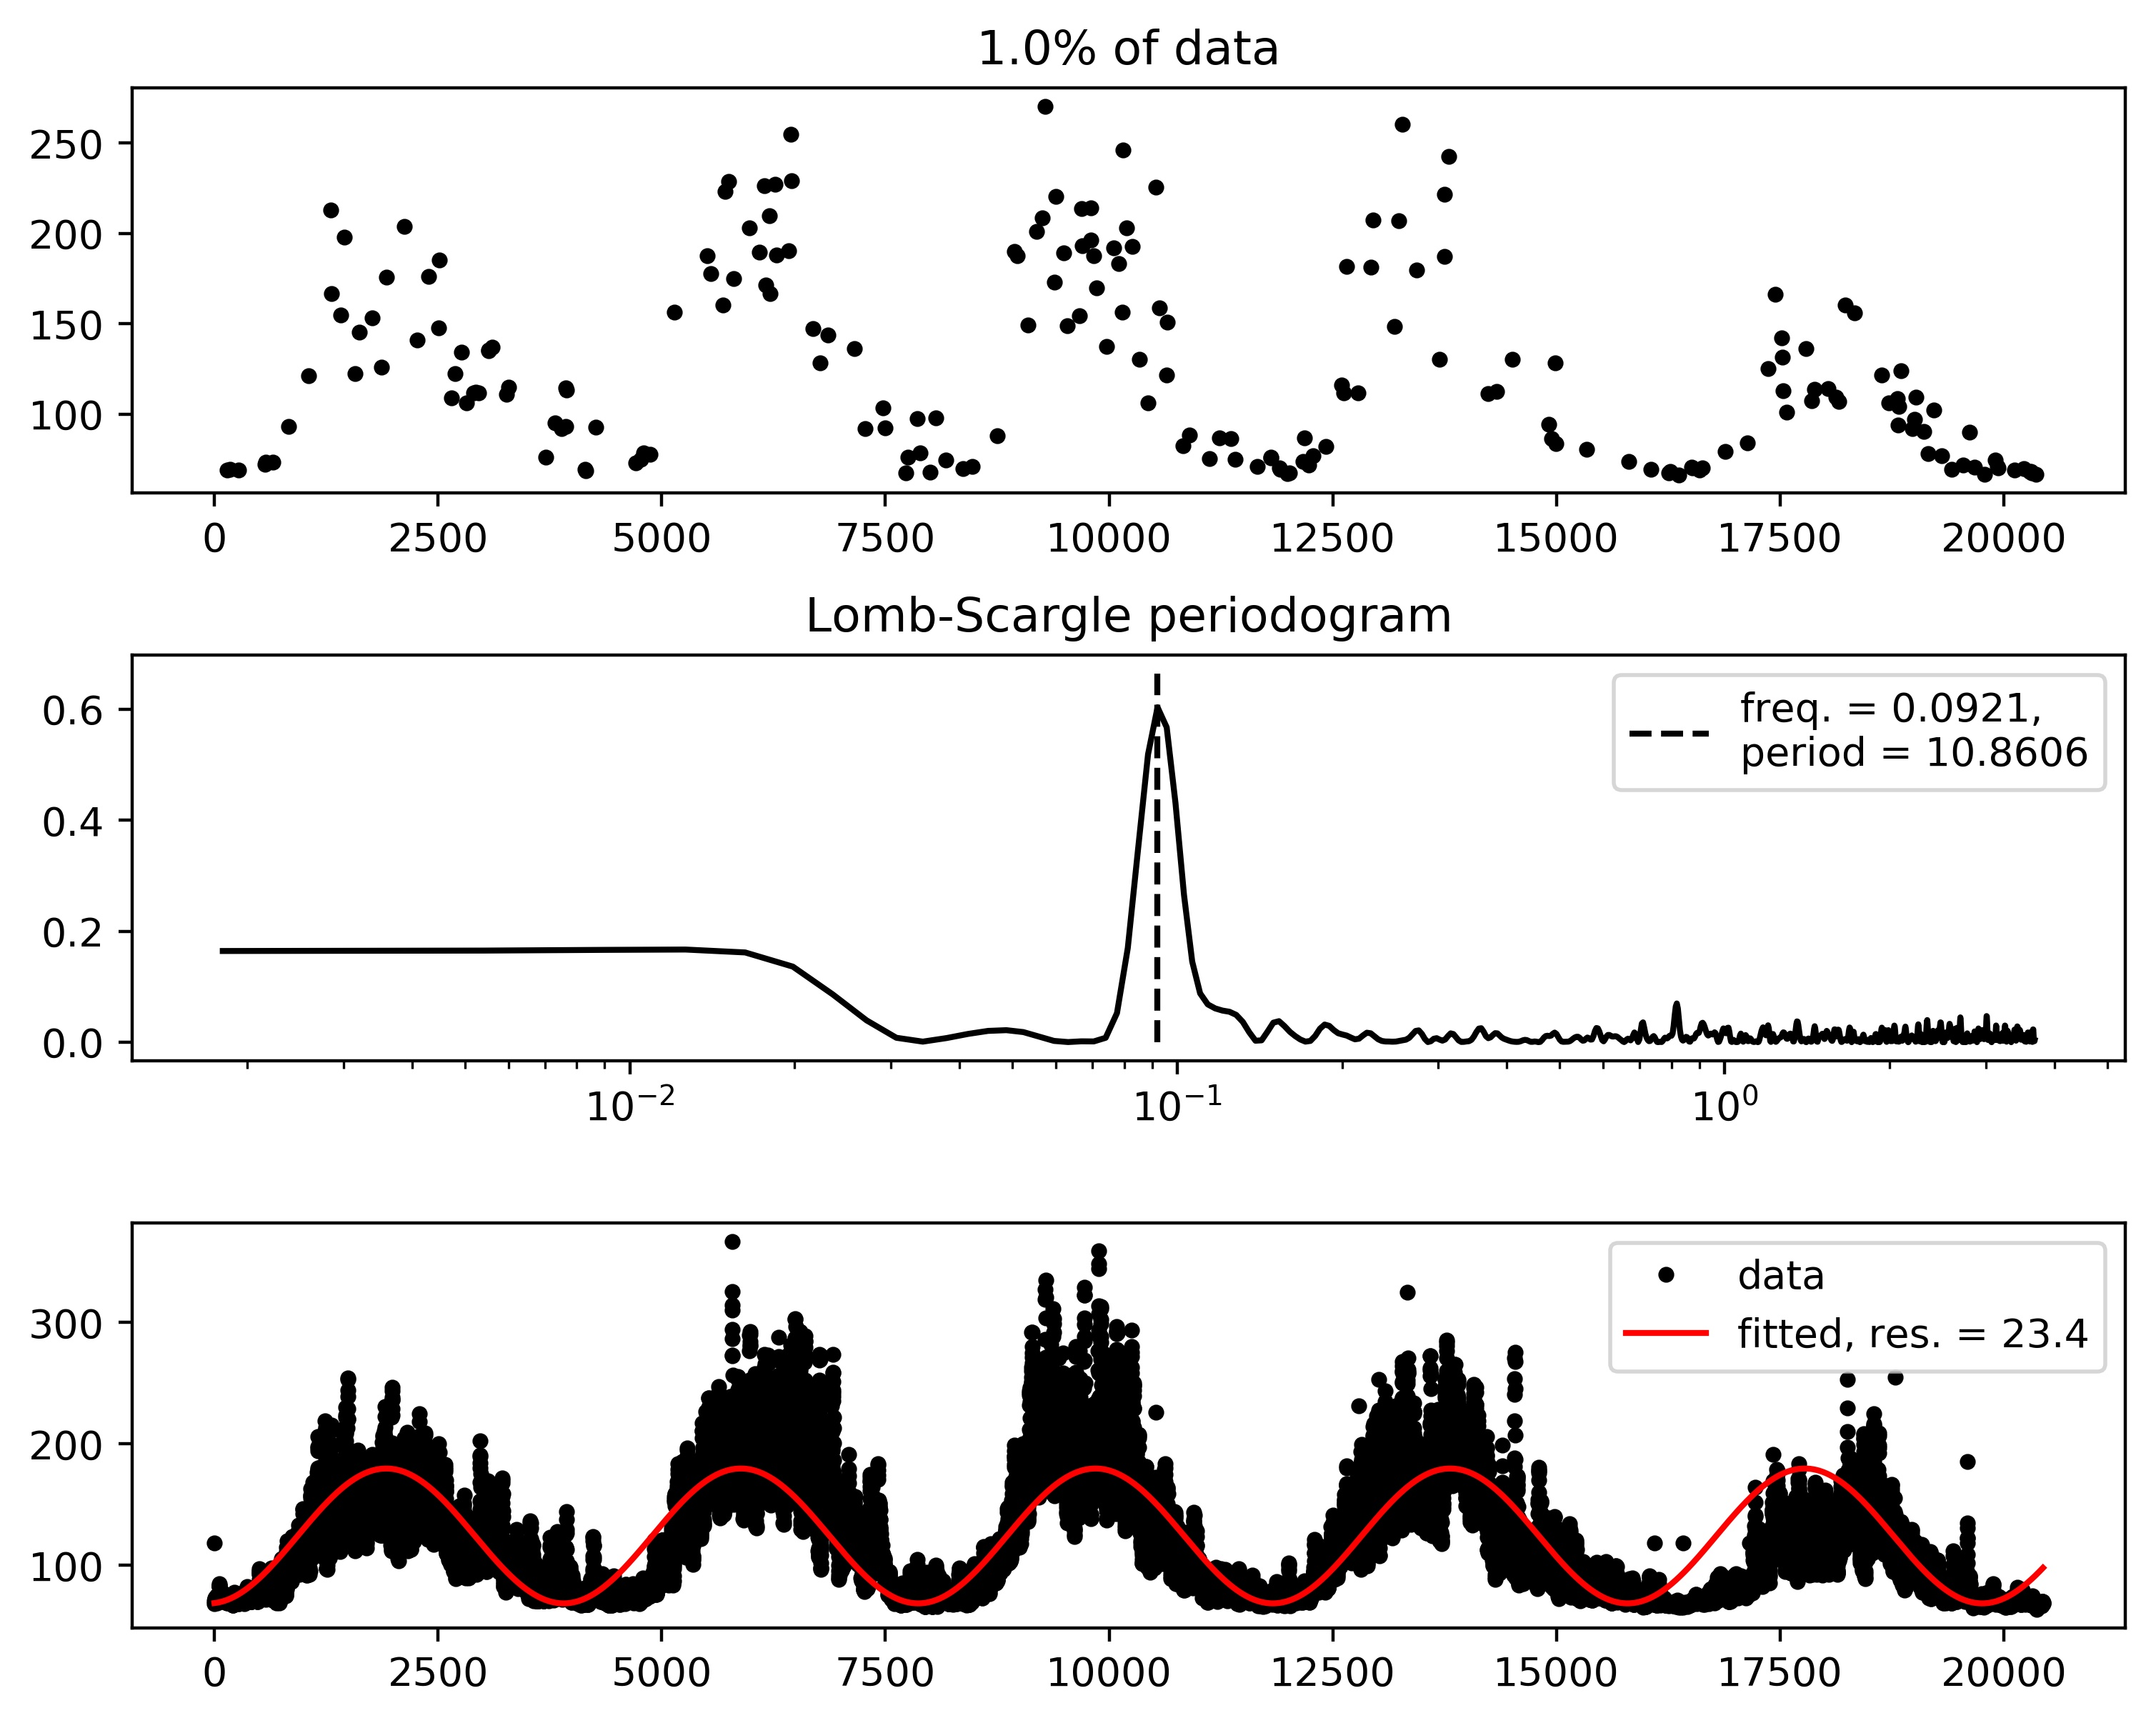
\includegraphics{../scripts/dataset1/periodograms_ny2.0_model1_pg0.99.jpg}}
	\end{center}
	\vspace{-1mm}	
	\legenda{A série original continha $\sim$20000 amostras, de modo que 1\% destes dados, ainda que aleatoriamente distribuídos, é capaz não só de indicar o formato original da série (graças aos nossos olhos e nossa capacidade de identificar padrões) mas também de ser analisada com excelência via periodograma de Lomb-Scargle (graças à classe \texttt{LoombScargle}).}
	\label{fig:percent1}
	\vspace{-8mm}	
\end{figure}

\begin{figure}[ht!]
\vspace{-14mm}	
	\caption{Análise com exclusão aleatória até 0.5\% dos dados.}
	\vspace{1mm}	
	\begin{center}
		\resizebox{.8\textwidth}{!}{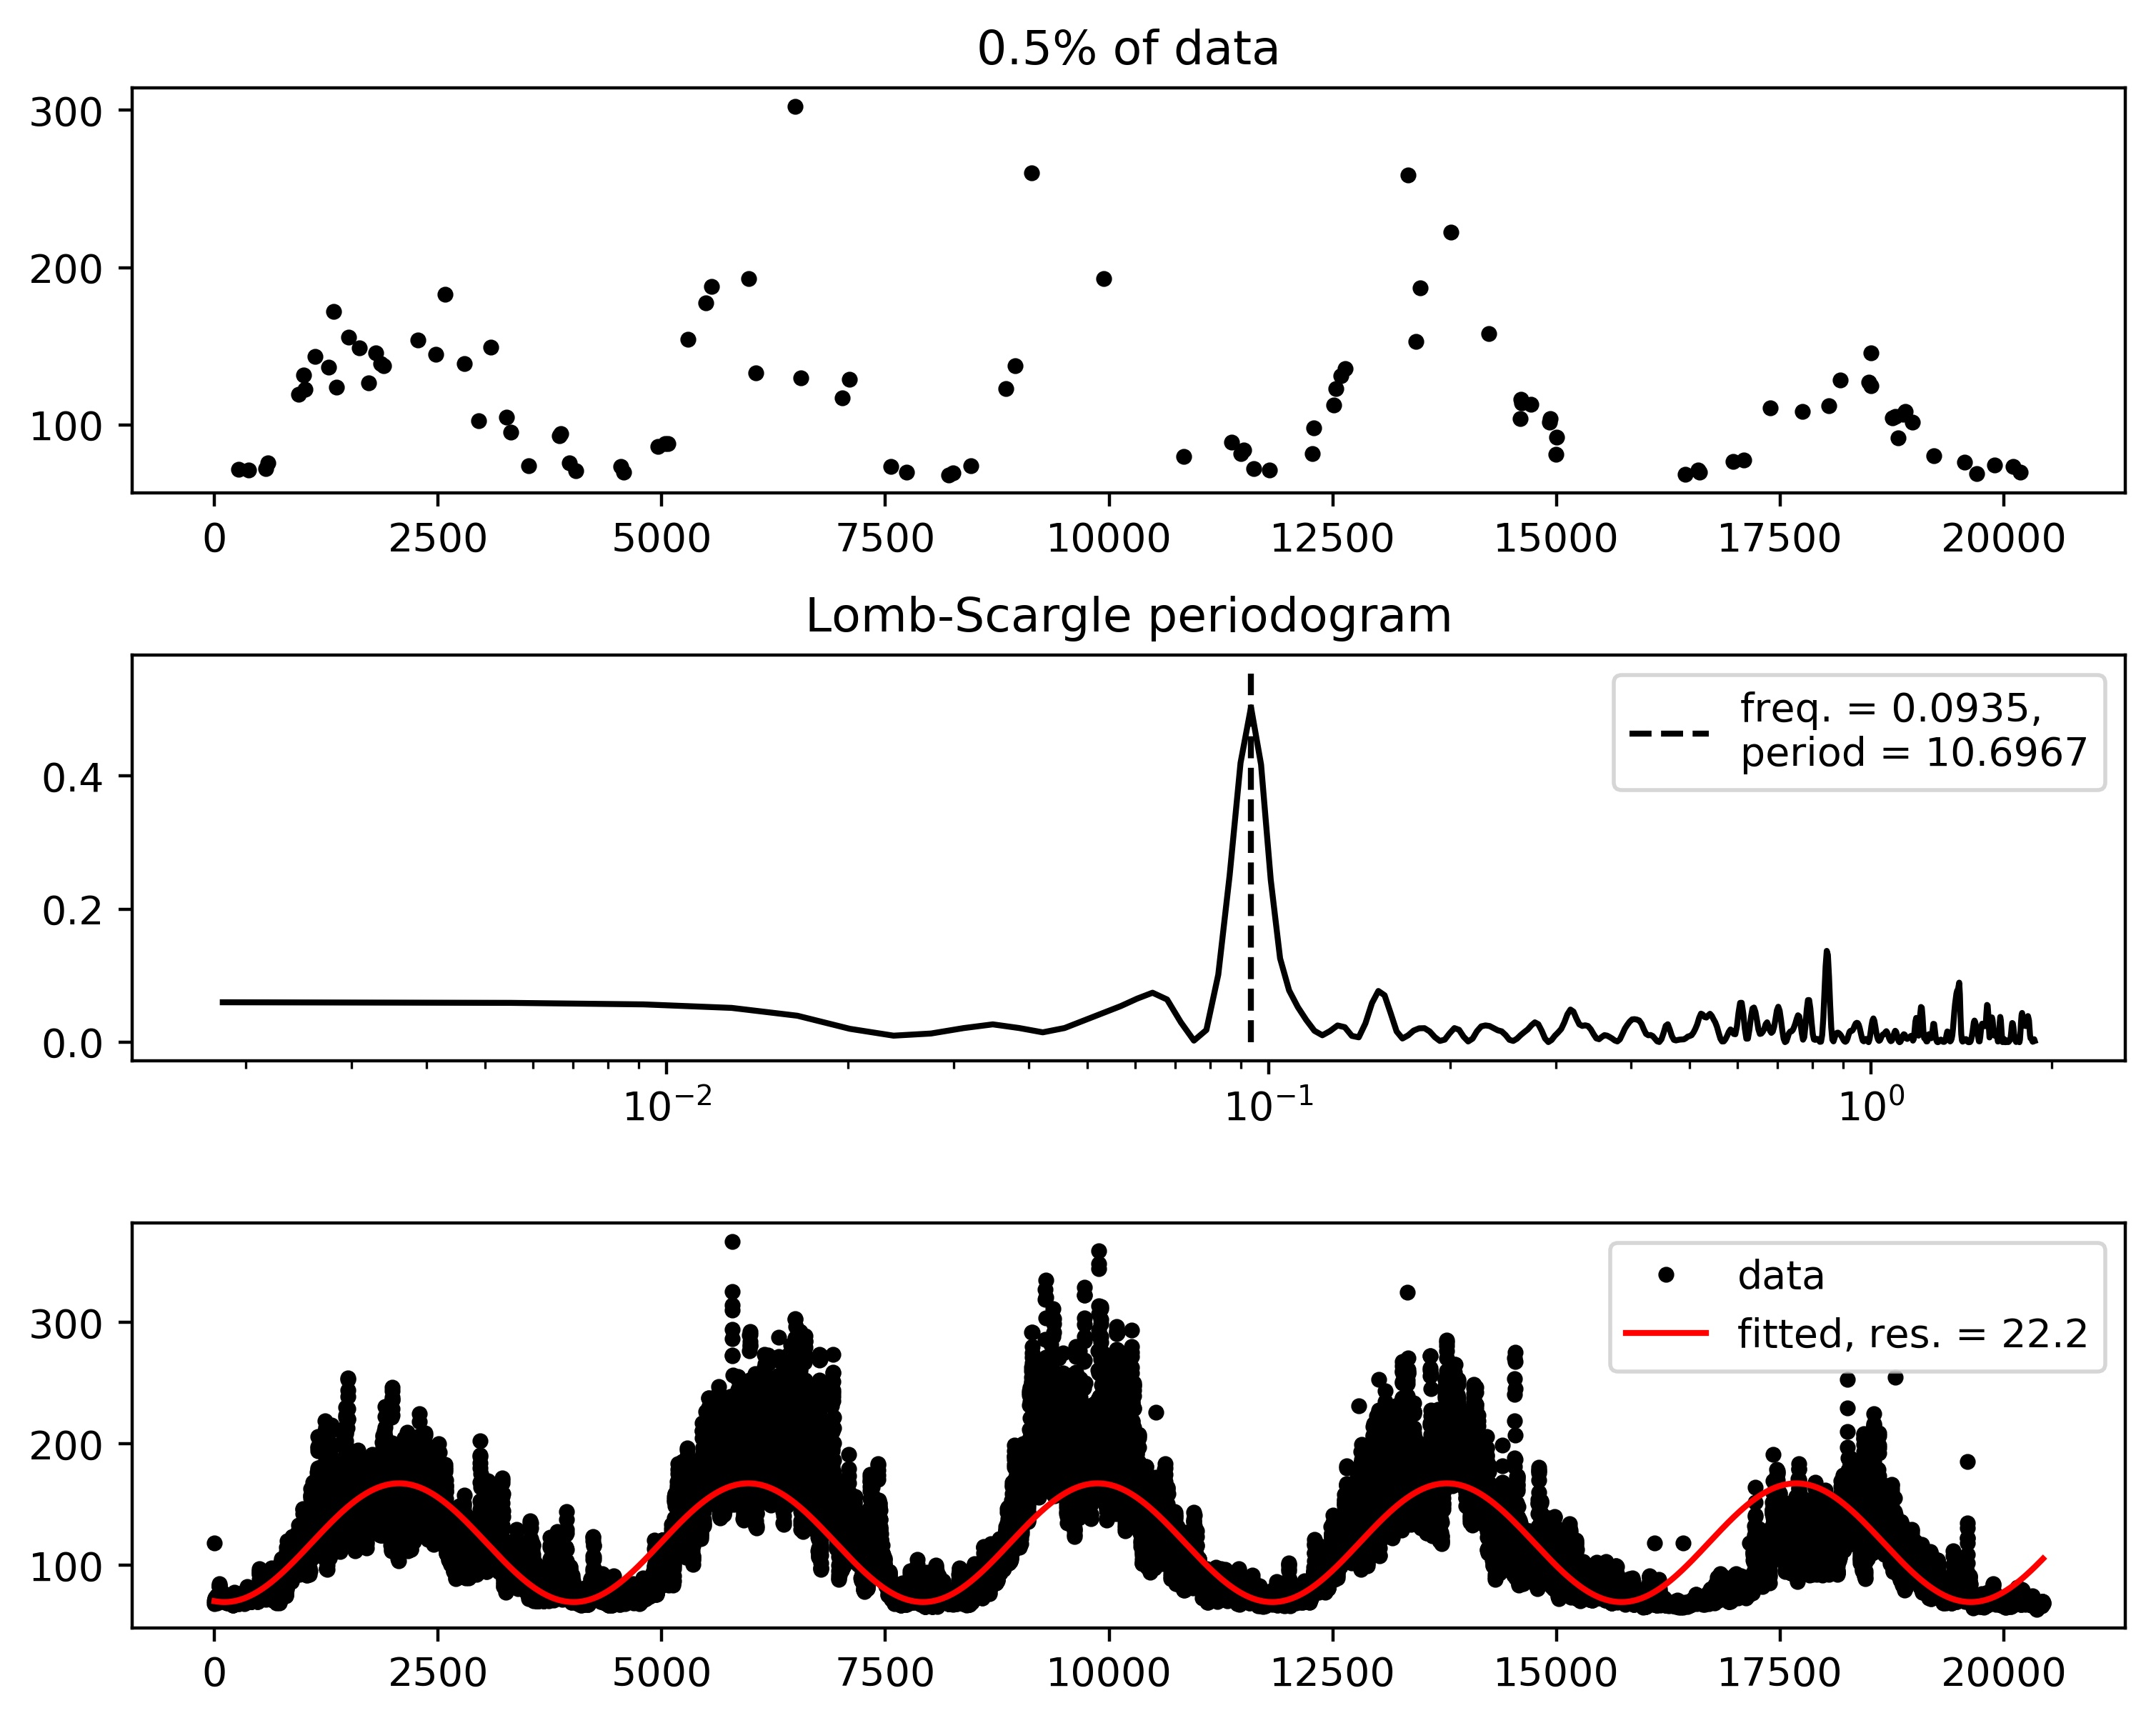
\includegraphics{../scripts/dataset1/periodograms_ny2.0_model1_pg0.995.jpg}}
	\end{center}
	\vspace{-1mm}	
	\legenda{Com 0.5\% dos dados a série se apresenta mais descaracterizada, mas com pontos suficientes para se assemelhar à a série original. O periodograma de Lomb-Scargle foi aplicado com sucesso.}
	\label{fig:percent0.5}
	\vspace{-3mm}
\end{figure}

\begin{figure}[ht!]
\vspace{-12mm}	
	\caption{Análise com exclusão aleatória até 0.1\% dos dados.}
	\vspace{1mm}	
	\begin{center}
		\resizebox{.8\textwidth}{!}{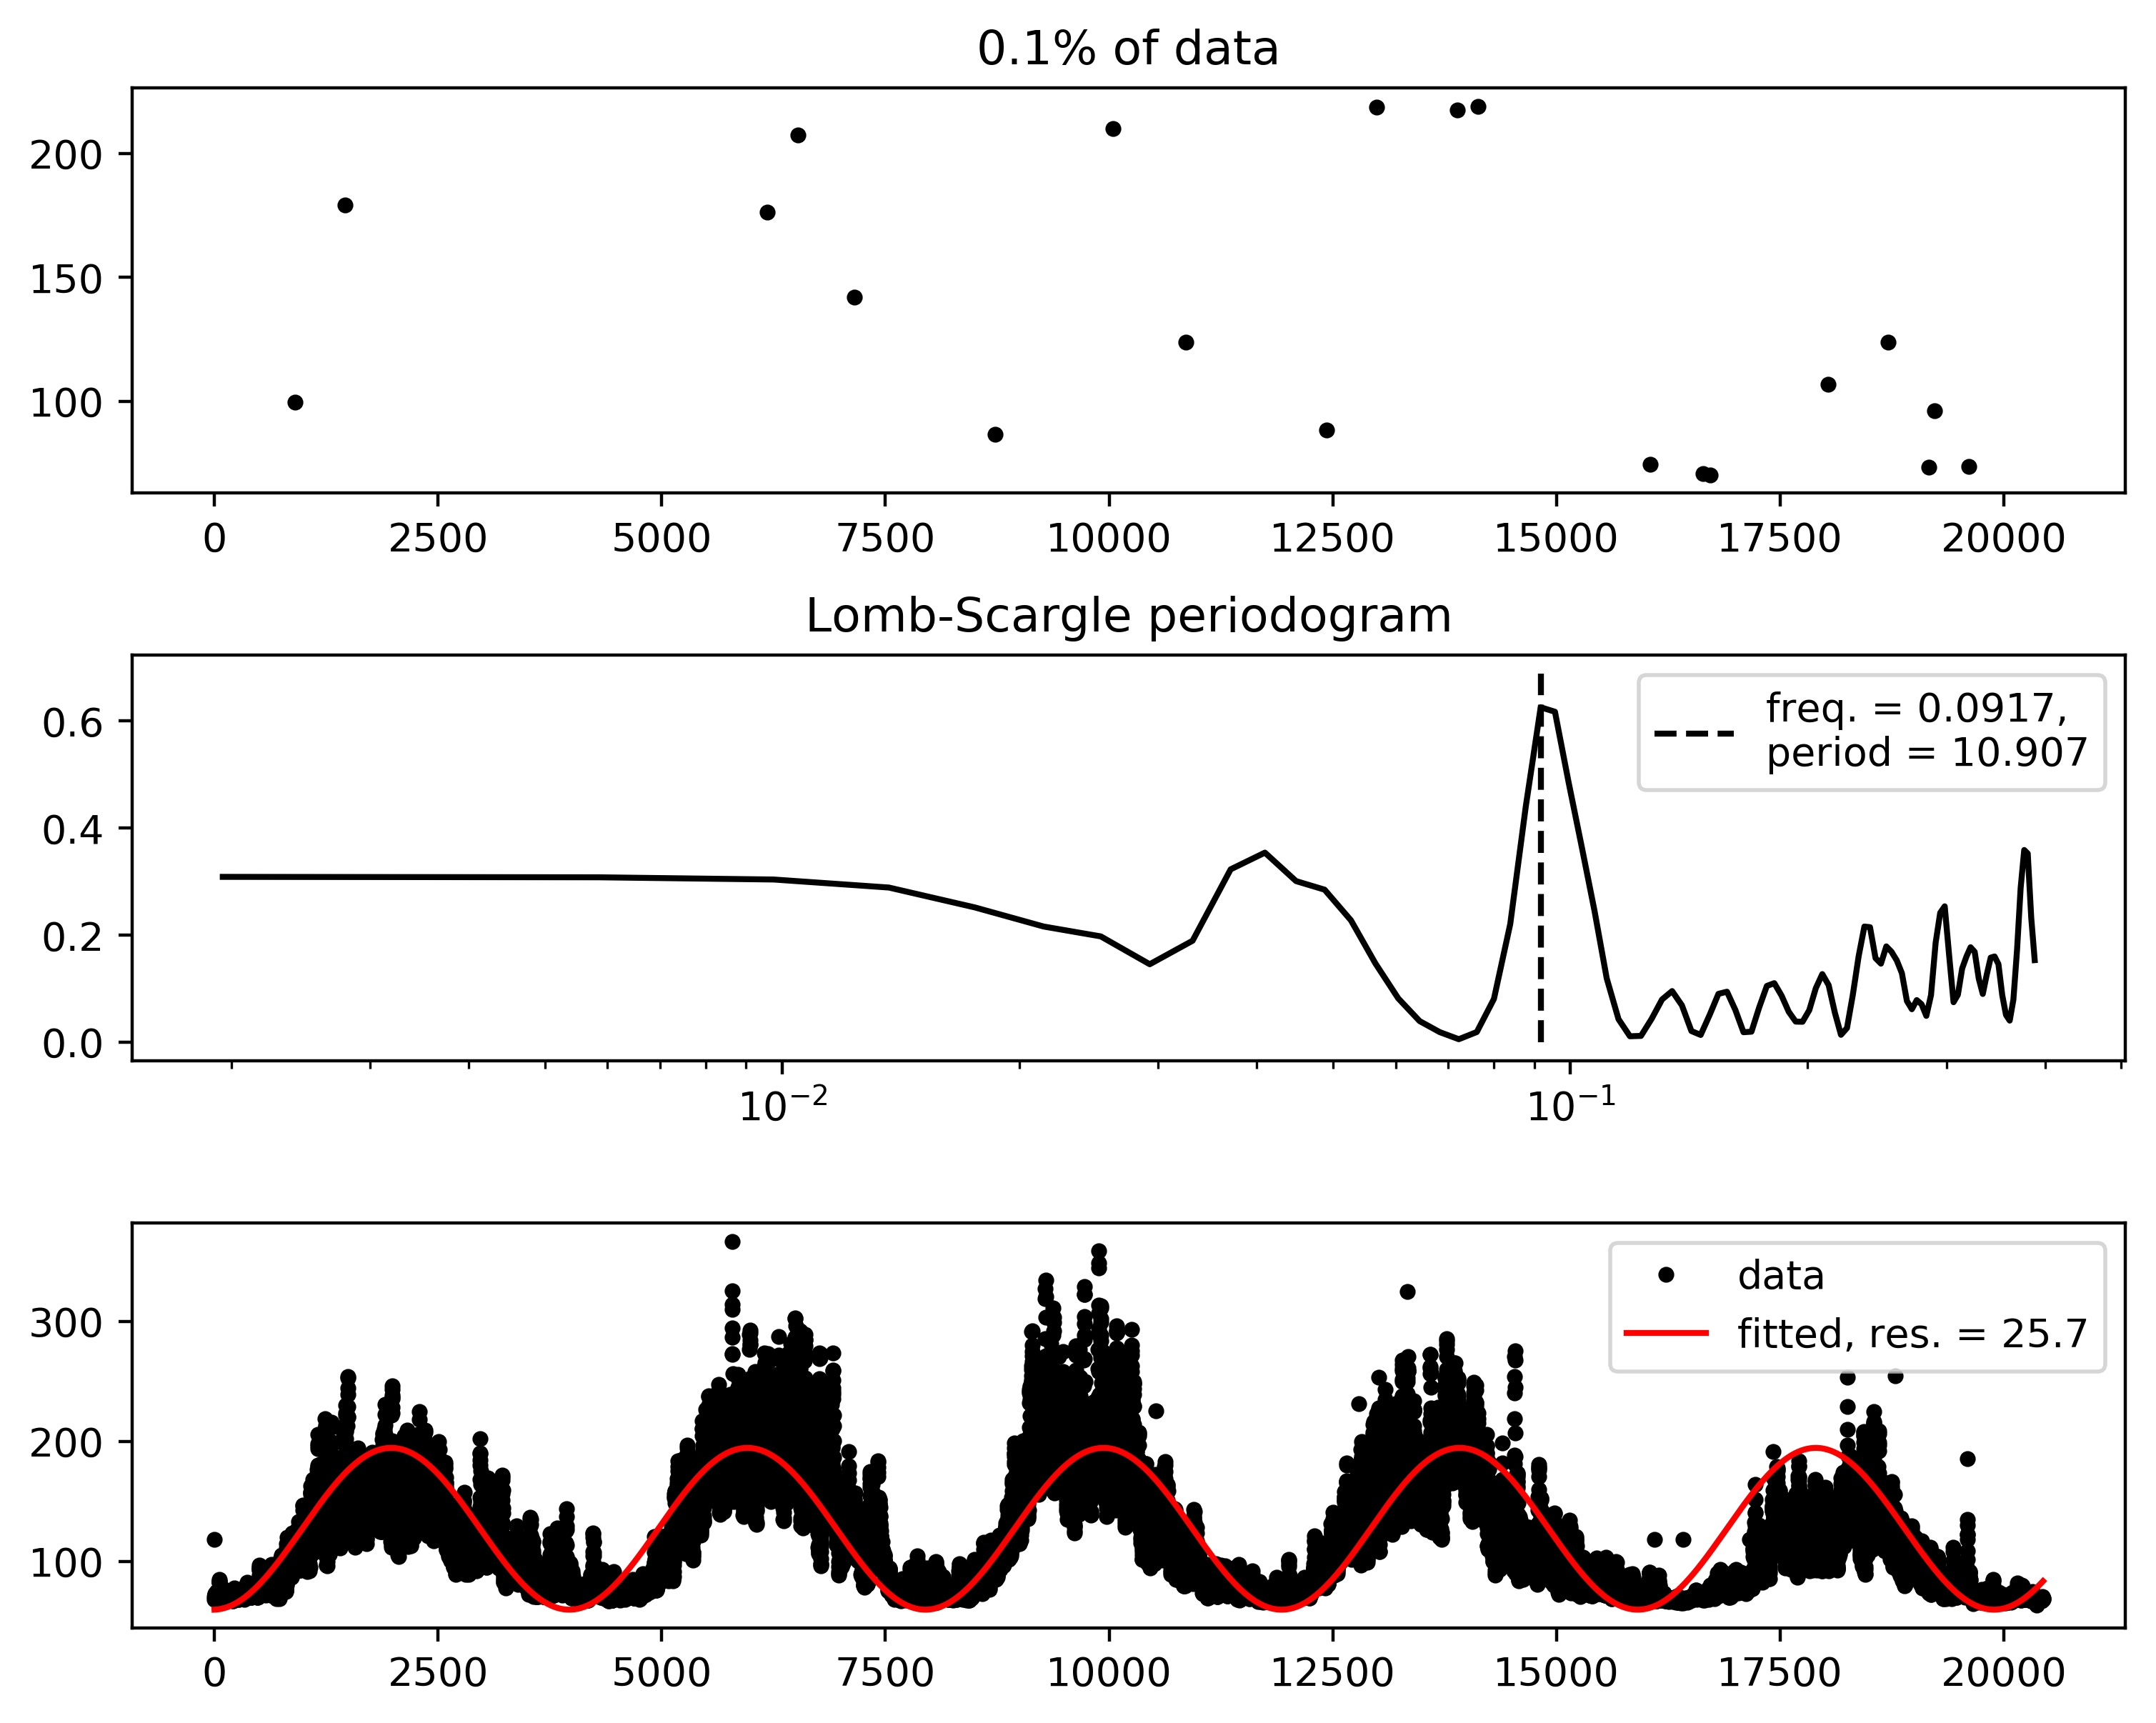
\includegraphics{../scripts/dataset1/periodograms_ny2.0_model1_pg0.999.jpg}}
	\end{center}
	\vspace{-1mm}	
	\legenda{Com somente 0.1\% dos dados, o perfil da série não é mais aparente e no periodograma surgem frequências espúrias. O período de $\sim$11 anos continua sendo corretamente determinado pela ferramenta.}
	\label{fig:percent0.1}
	\vspace{-5mm}	
\end{figure}

\begin{figure}[ht!]
\vspace{-10mm}	
	\caption{Análise com exclusão aleatória até 0.05\% dos dados.}
	\vspace{1mm}	
	\begin{center}
		\resizebox{.8\textwidth}{!}{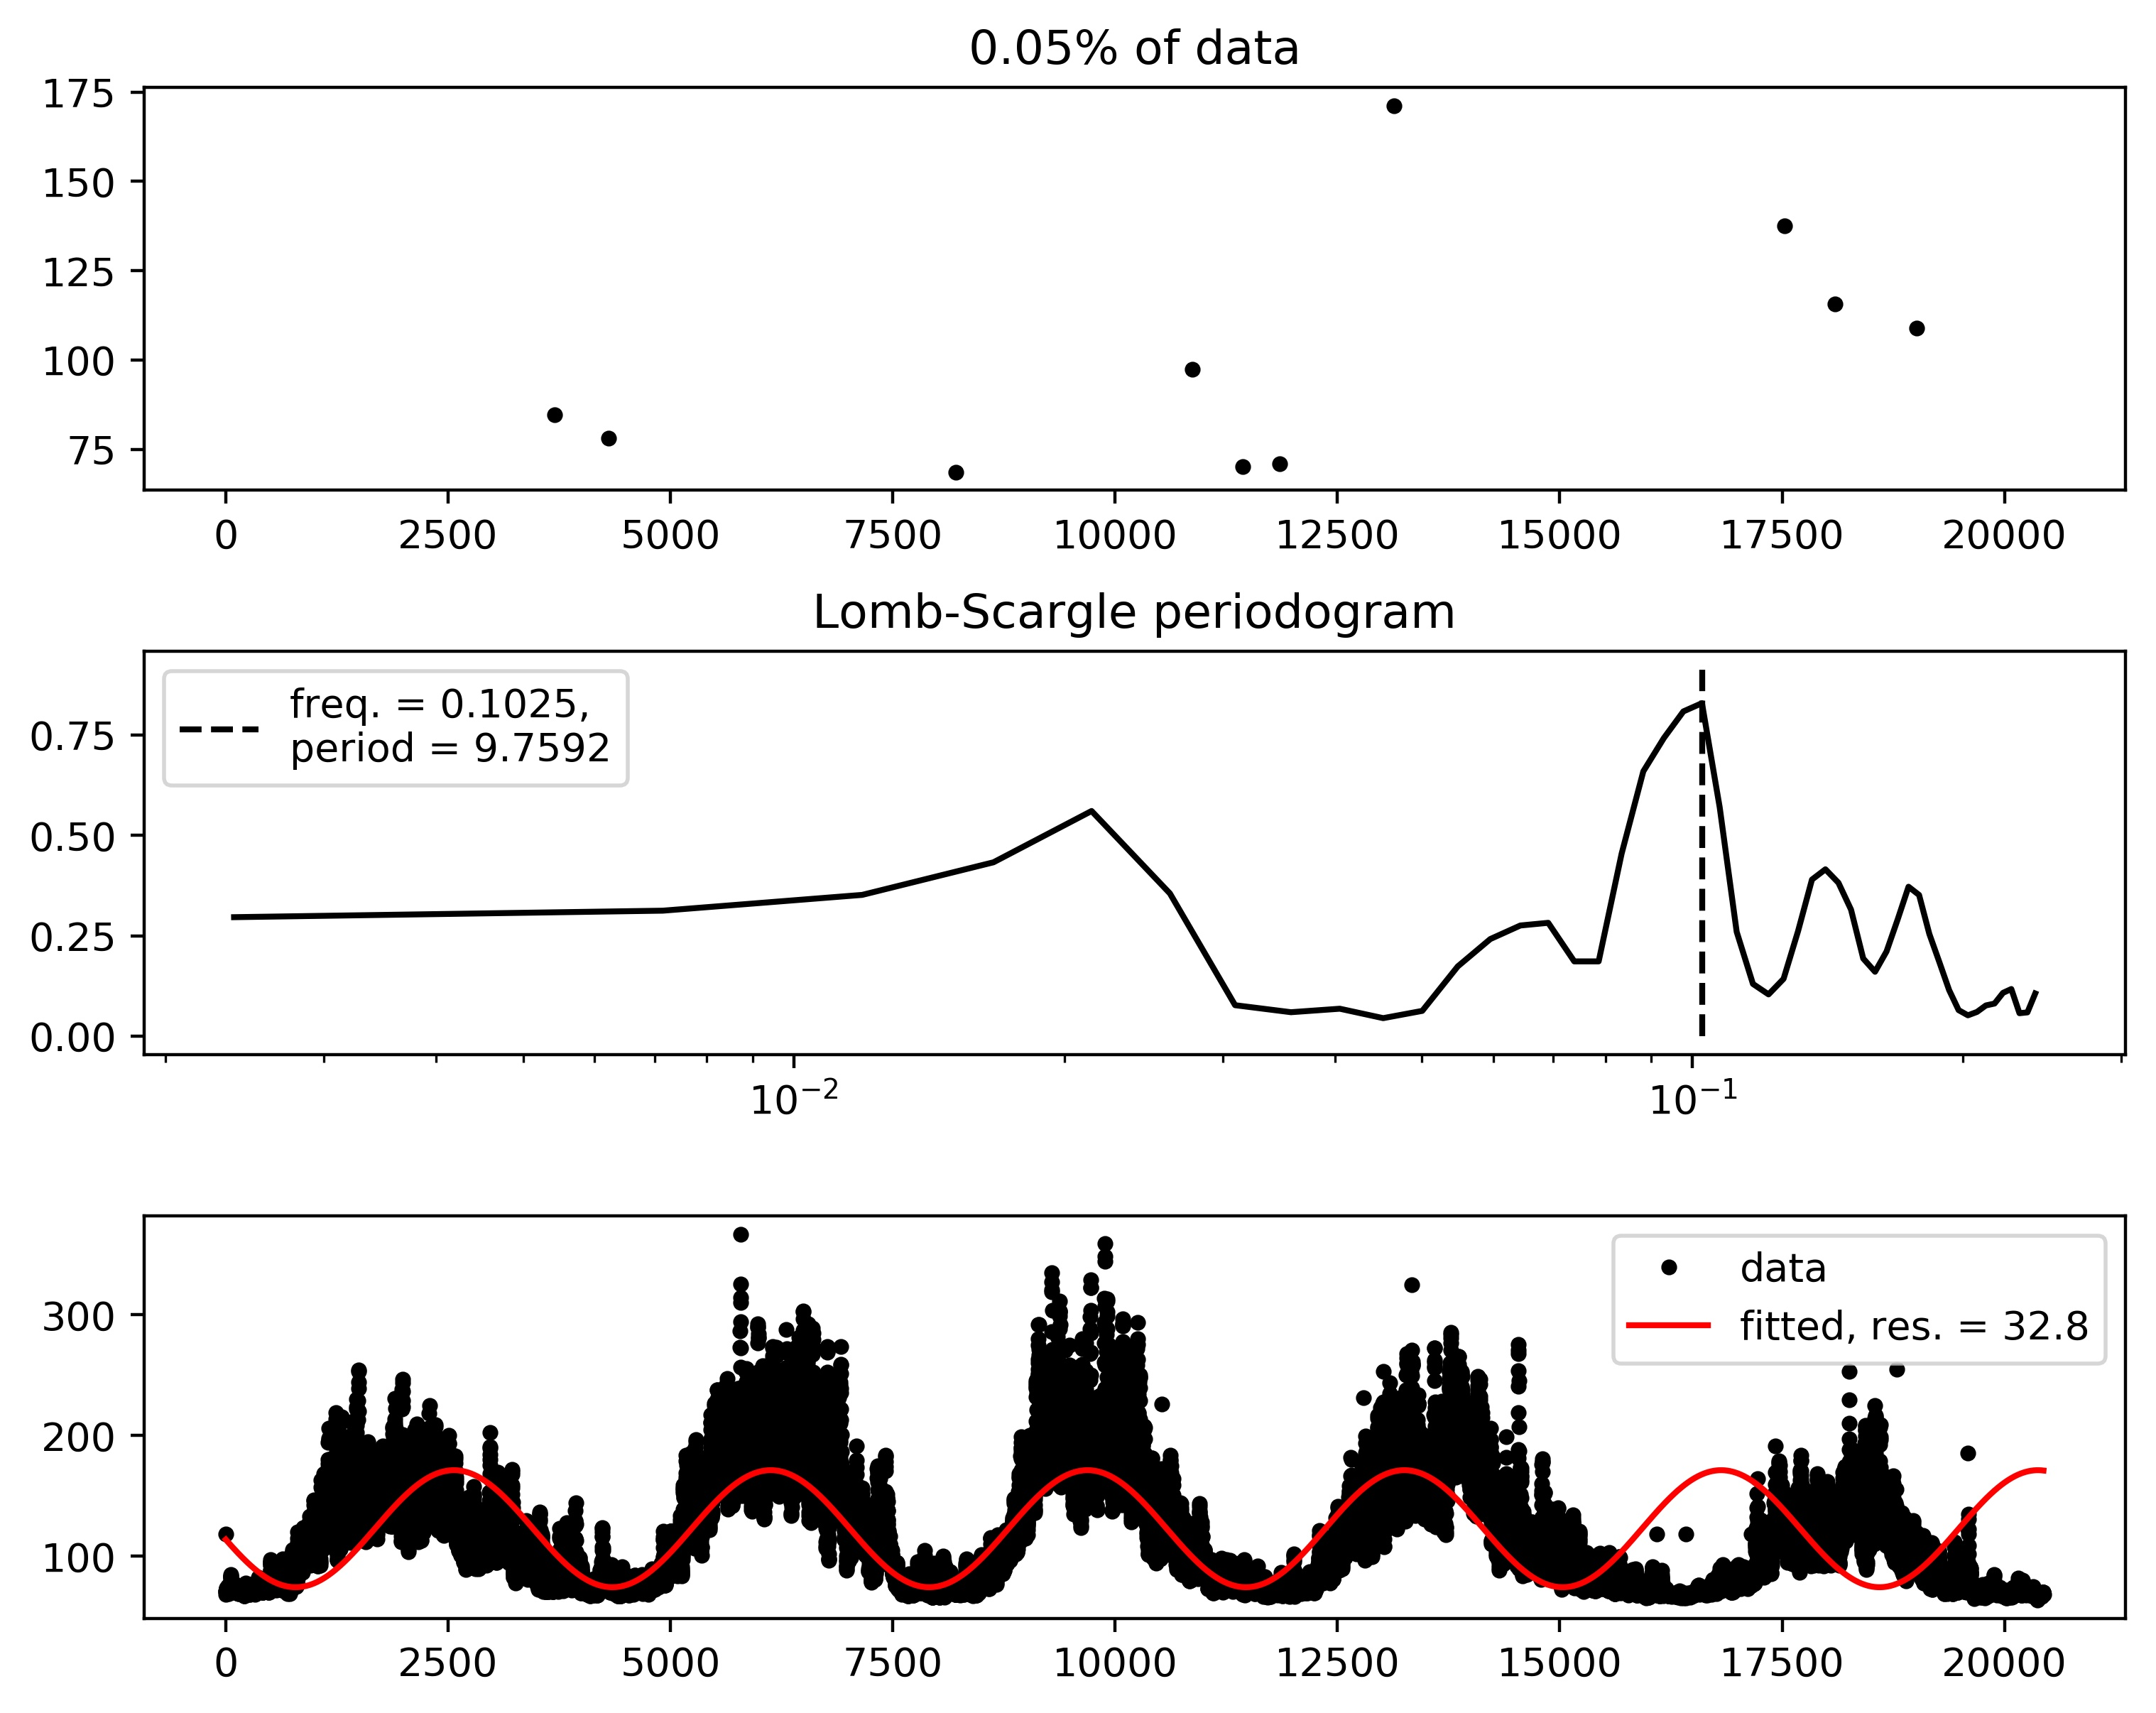
\includegraphics{../scripts/dataset1/periodograms_ny2.0_model1_pg0.9995.jpg}}
	\end{center}
	\vspace{-1mm}	
	\legenda{Aqui o periodograma de Lomb-Scargle apresenta seus picos com baixa resolução (picos espalhados). Ainda assim, a frequência determinada é satisfatória e a senóide resultante se ajusta bem à série, conforme ilustrado pelo plot de baixo.}
	\label{fig:percent0.05}
\end{figure}

\begin{figure}[ht!]
\vspace{-10mm}	
	\caption{Análise com exclusão aleatória até 0.04\% dos dados.}
	\vspace{1mm}	
	\begin{center}
		\resizebox{.8\textwidth}{!}{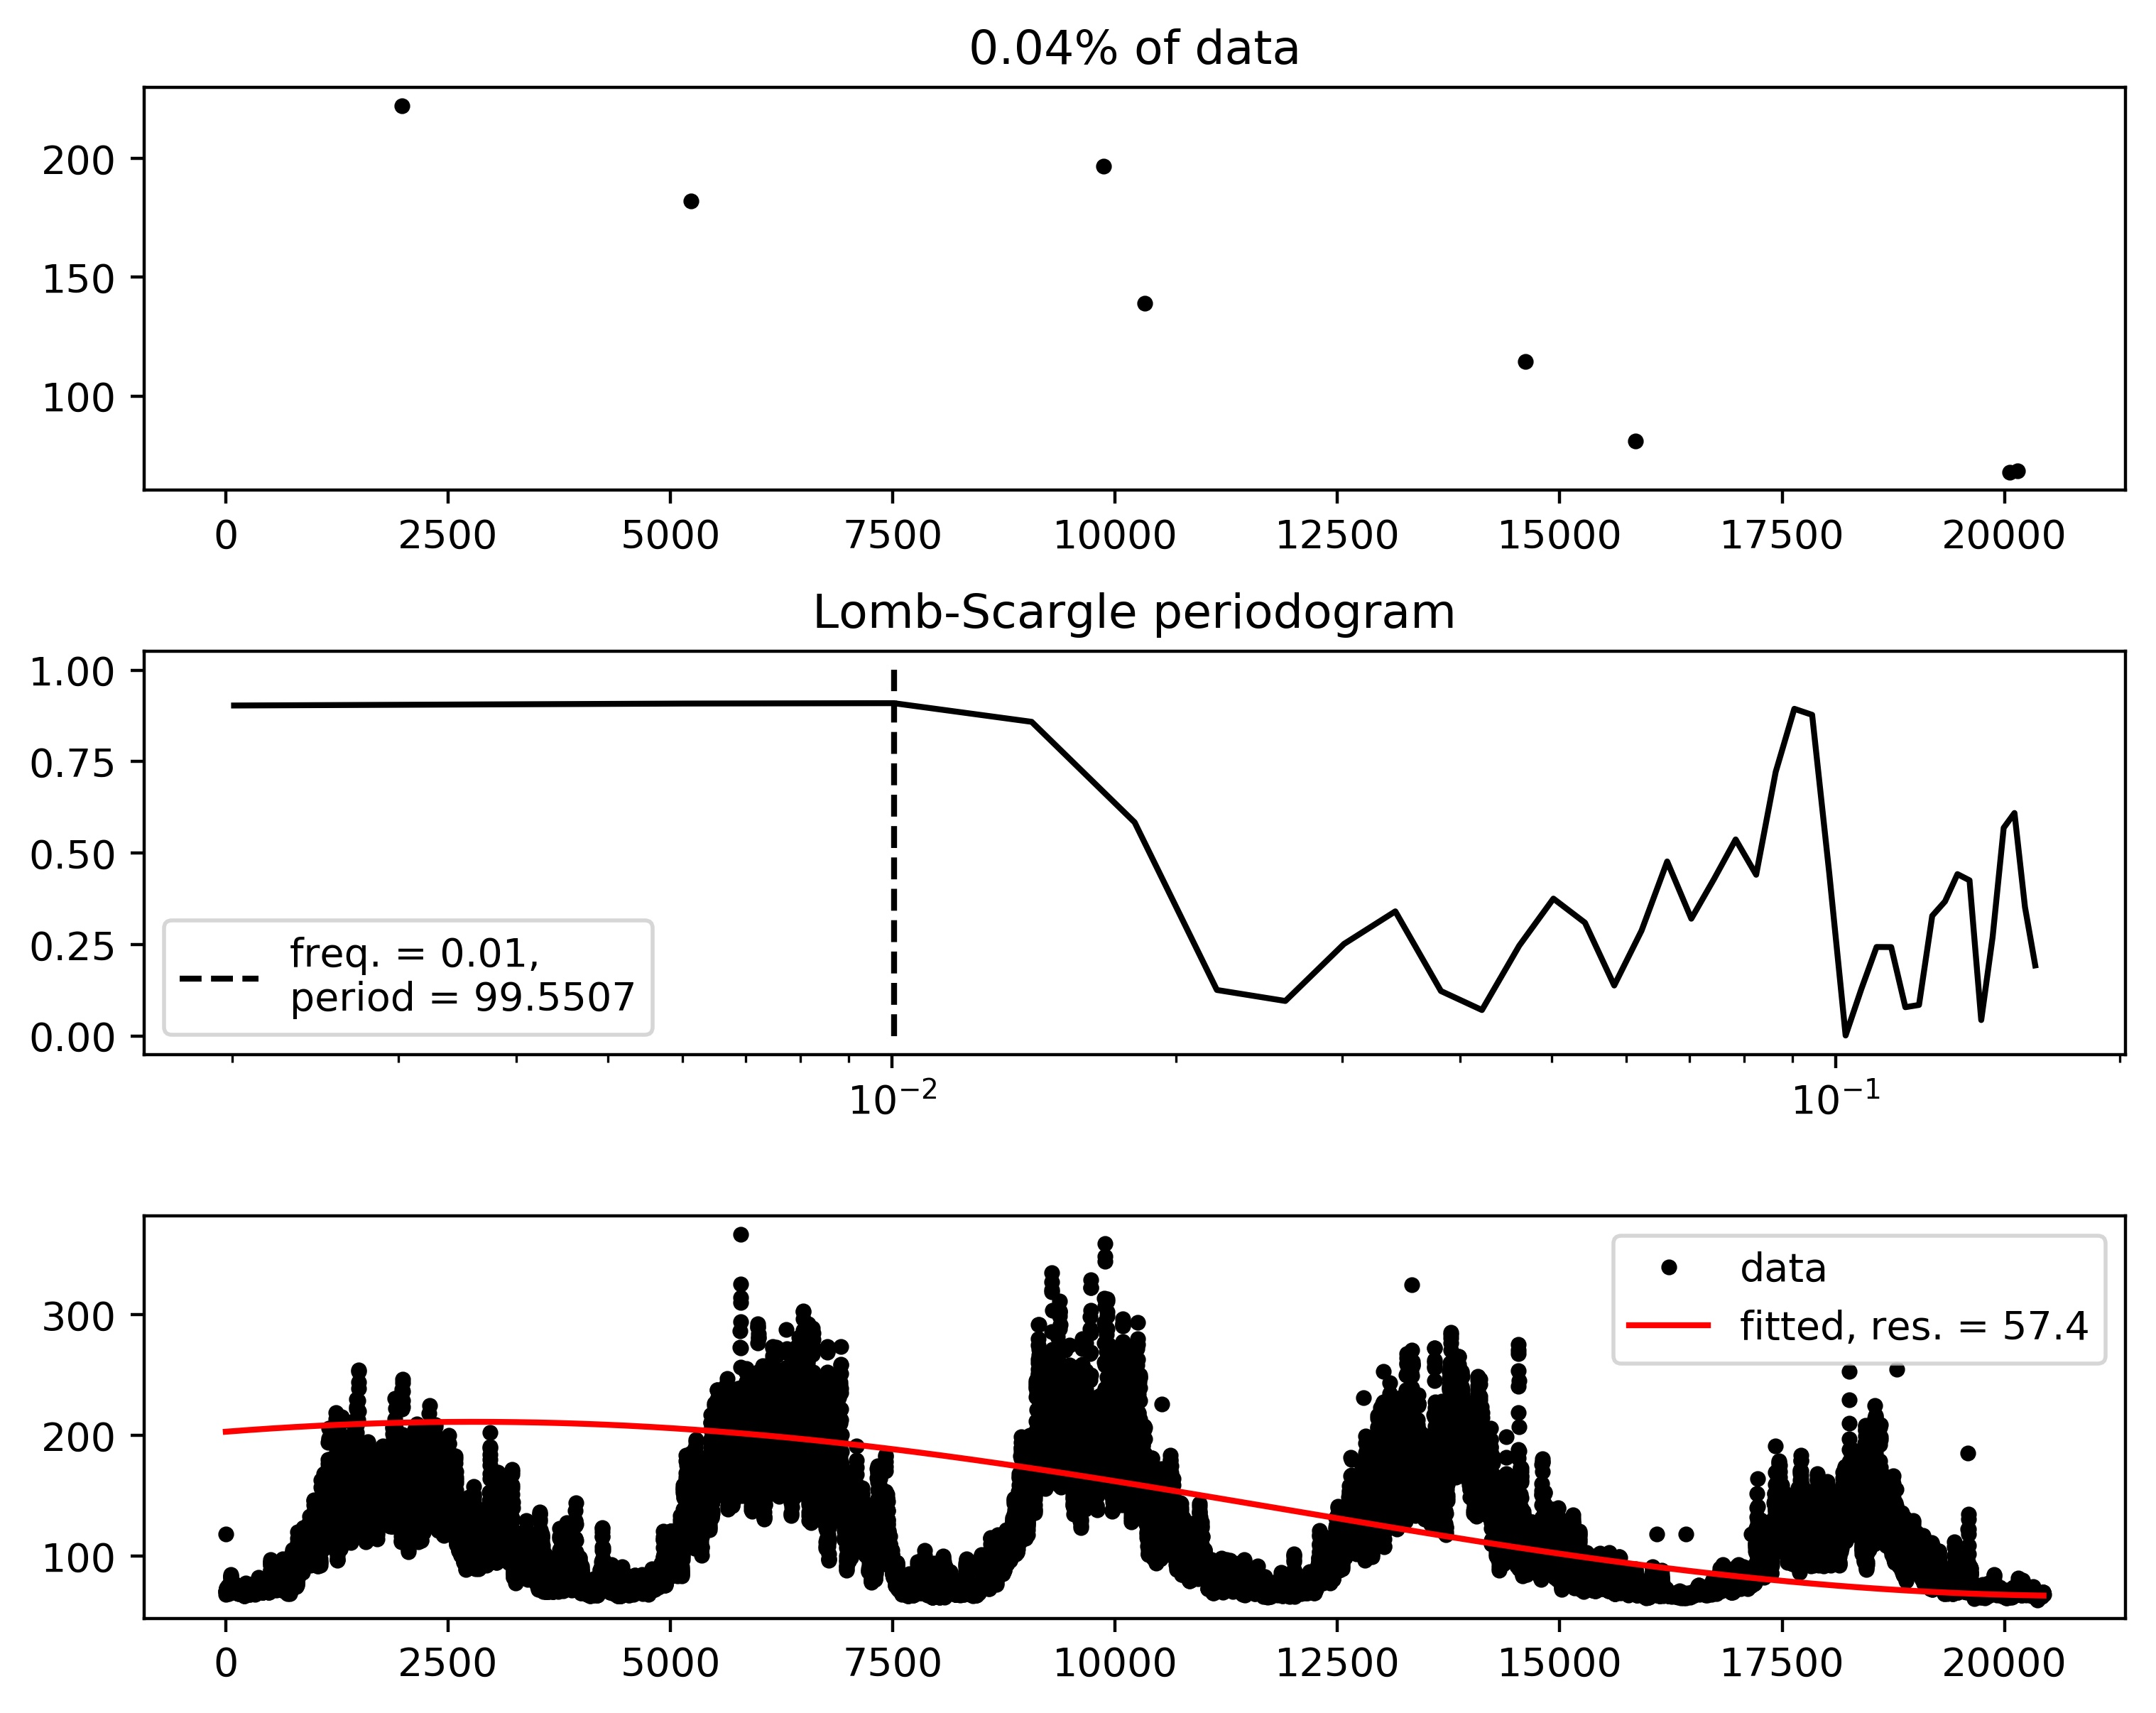
\includegraphics{../scripts/dataset1/periodograms_ny2.0_model1_pg0.9996.jpg}}
	\end{center}
	\vspace{-1mm}	
	\legenda{Neste teste, com 0.04\% dos dados, o periodograma de Lomb-Scargle falhou. A assinatura da série é completamente perdida, e a função ajustada é completamente diferente do esperado.}
	\label{fig:percent0.04}
\end{figure}

\clearpage{}
Para os fins desta discussão, considera-se um bom resultado do \texttt{LombScargle} um periodograma suave, próximo de zero em todas as frequências a não ser pela presença de um pico na frequência conhecida de 0.089 ou próximo desta, e com pouca ou nenhuma frequência espúria. A Figura \ref{fig:percent1} (experimento com 1\% dos dados), se contrastada com as Figuras \ref{fig:4gaps} a \ref{fig:8gaps}, indica que a baixa quantidade de dados não necessariamente afeta a performance da ferramenta. Em outras palavras, o resultado sob as condições da Figura \ref{fig:percent1} foi tão bom ou melhor que sob as condições de todos os testes do cenário anterior. O teste com 0.5\% (Figura \ref{fig:percent0.5}) obteve um resultado tão bom quanto o teste anterior. O teste com 0.1\% dos dados (Figura \ref{fig:percent0.1}) foi particular: mesmo quando o perfil oscilatório (visual) dos dados está totalmente perdido, o uso do \texttt{LombScargle} permitiu recuperar com êxito a característica original do sinal. Abaixo de 0.1\%, assim como durante os testes do cenário anterior, a performance da ferramenta caiu demasiadamente e se tornou igualmente inconsistente para todos os valores. Ou seja, a depender dos dados aleatoriamente excluídos, o resultado da ferramenta era o mesmo com 0.05\% (Figura \ref{fig:percent0.05}) ou 0.04\% (Figura \ref{fig:percent0.04}) dos dados, e estes eram muito piores que os resultados com 0.1\% dos dados ou mais.

